% Pr�ambel
%====================================================================================================================
% Headerdatei f�r einen Bericht
%====================================================================================================================

%====================================================================================================================
% Die KOMA-Skript Dokumentklasse "scrreprt" verwenden

\documentclass[
		english,
		% eine der beiden folgenden Optionen ausw�hlen:
		final,				% hiermit wird die endg�ltige Fassung des Dokuments erstellt
%		draft,				% hiermit wird eine Rohfassung erstellt, 
									% in der die Bilder nur als Rahmen erscheinen und schwarze Balken neben
									% �bervolle Boxen gezeichnet werden
		pdftex,				% automatische PDF-Verlinkung, bessere Bildereinbindung
		12pt,					% Standardschriftgr��e
		fleqn,				% Formeln linksb�ndig
		a4paper,			% DIN-A4-Papier
		titlepage,		% extra Titelseite verwenden
		numbers=noenddot, % �berschriften ohne Punkt (nach DIN eigentlich mat, wenn auch Buchstaben verwendet werden)
		bibliography=totoc			% Literaturverzeichnis im Inhaltsverzeichnis
		%chapterprefix	% "Kapitel x" zus�tzlich
]{scrreprt}
\pdfoptionpdfminorversion=5 % akzeptiere auch Bilder in PDF Version 1.5

%====================================================================================================================
% Pakete laden

% Seitenr�nder und Kopf-/Fu�zeilen einstellen
\usepackage[a4paper,
	headsep=0.5cm,
	footskip=0.8cm,
	left=3.5cm, right=2.5cm,
	top=2.5cm, bottom=2.0cm]{geometry}
% TEST: Blattgeometrie auf der ersten Seite anzeigen
%\geometry{showframe}

% Intelligente Verweise (mit automatischer Erg�nzung von "auf Seite XX")
% Achtung, nicht nach hyperref laden!!!
% wird aktiviert, falls \vref statt \ref benutzt wird
\usepackage{varioref}

% Kopf- und Fu�zeilen ver�ndern
\usepackage{fancyhdr}
\pagestyle{fancy}
% Kopfzeile: Lehrstuhlsschriftzug links, Logo rechts
\lhead{\sffamily{\Large Lehrstuhl f�r Steuerungs- und Regelungstechnik\\ \small Technische Universit�t M�nchen}}
\rhead{
\includegraphics[height=1.25cm]{pics/lsr_logo.png}}
\setlength{\headheight}{40pt}
% erh�hten Platz f�r Kopfzeile ber�cksichtigen
\addtolength{\textheight}{12pt}         % alte H�he dazu
\addtolength{\textheight}{-\headheight} % und neue wieder abziehen

% Folgende Befehle einkommentieren, um Abs�tze durch Abst�nde zu trennen
% Werden sie auskommentiert, so beginnt jeder Absatz mit einem Erstzeileneinzug
% Einzug bei Absatzbeginn
\parindent=0cm
% Abstand zwischen Abs�tzen (hier gleich Zeilenabstand)
\parskip=\baselineskip

% Deutsche Trennungen, Anf�hrungsstriche und mehr:
\usepackage[german english]{babel}
%\usepackage{english}

% Umlaute direkt eingeben (�,�,�)
% Auf Linuxsystemen hier eher utf-8 statt latin1
\usepackage[utf8]{inputenc}

% intern: � gleich als ganzes Zeichen darstellen und nicht aus ^ und a zusammensetzen
\usepackage[T1]{fontenc}

% Zum Einbinden von Graphiken
\usepackage{graphicx}
\graphicspath{{pics/}}

% Mathematische Symbole f�r
\usepackage{amsmath}
\usepackage{amssymb}

% Automatische Erstellung eines Symbolverzeichnisses
% Dazu muss ein spezieller MakeIndex-Lauf nach jedem Erstellen erfolgen, 
% siehe Dokumentation zu nomencl und nomentbl
\usepackage[german]{nomentbl}
\makenomenclature

% Deutsche BiBTeX-Styles nach DIN 1505
\usepackage{bibgerm}
% \bibliographystyle{alphadin}          % alphabetische K�rzel
\bibliographystyle{plaindin}				% numerische K�rzel

% verlinktes Inhaltsverzeichnis, logische Seitenzahlen im PDF etc.
\usepackage[
	plainpages=false, 
	pdfpagelabels, 
	colorlinks=false, % true: Links werden farbig gedruckt (Bildschirm-Version) 
	                  % false: Links werden schwarz gedruckt, haben aber bunte Box auf dem Bildschirm (Druckversion)
	linkcolor=blue,   % Farbe f�r interne Links
	final]
	{hyperref}
	
% Pakete von Sch�lls Beispiel
\usepackage{longtable}            % F�r evtl. mehrseitige Tabellen
\RequirePackage{array}
\usepackage{dcolumn}              % in Tabellen an Dezimaltrennzeichen ausrichten
\newcolumntype{.}[1]{D{.}{.}{-1}} % neuer Spaltentyp: .{} richtet am Dezimalpunkt zentriert aus
\newcolumntype{d}[1]{D{.}{.}{#1}} % neuer Spaltentyp: d{x} richtet am Dezimalpunkt mit x Nachkommastellen aus

\usepackage{subfig}               % F�r mehrteilige Abbildungen
\usepackage{textcomp}             % F�r diverse Sonderzeichen, u.a. \textdegree f�r Gradzeichen
\usepackage{booktabs}             % F�r schicke Linien in z.B. Tabellen
\usepackage[subfigure]{tocloft}   % Erstellen eigener Verzeichnisse, ben�tigt f�r das TODO-Makro
\usepackage{ifthen}               % Entscheidungen im Quellcode
\usepackage{color}                % in Farbe uund buuuunt!

% Korrektes Setzen von Ma�einheiten, Zahlen u. a.
\usepackage[per-mode=symbol]{siunitx}

% Ein paar Einstellungen f�r das zu produzierende PDF
\hypersetup{
  pdfproducer={\pdftexbanner},
  bookmarksnumbered=true,
  bookmarksopen=false,
}

\usepackage{listings}
\usepackage[font={small,color=black}, labelfont=bf,figurename=Abb.]{caption} 
\usepackage{pxfonts}

\usepackage{pgfplots}
\usepackage{filecontents}
\usepackage[miktex]{gnuplottex}

\usepackage{wrapfig}


\newcommand{\shellcmd}[1]{\indent\indent\texttt{\scriptsize\# #1}}

% eigene Befehle
%========================================================================================================
% Eigene Befehle

% Mathematische Schreibweisen
% Vektoren: fettgedruckt (auskommentieren, um Vektoren mit Pfeil zu erhalten)
\renewcommand{\vec}[1]{\boldsymbol{#1}}
% Matrizen: auch fettgedruckt
\newcommand{\mat}[1]{\boldsymbol{#1}}
% partielle Ableitung
\newcommand{\partder}[2]{\frac{\partial #1}{\partial #2}} 
% Br�che mit schr�gem Bruchstrich
\newcommand{\nfrac}[2]{
  \leavevmode\kern.1em%
  \raise.5ex\hbox{\scriptsize #1}%
  \kern-.1em/\kern-.15em%
  \lower.25ex\hbox{\scriptsize #2}
}

% Todo-Anmerkungen machen und auflisten
\newcommand{\todolistname}{To Do:}
\newlistof{todo}{todo}{\todolistname}
\newcommand{\todo}[1] {%
  \refstepcounter{todo}
  \textbf{\color{red} TODO: #1!}
  \addcontentsline{todo}{todo}{#1}\par}

% Verweise auf Gleichungen, Abbildungen, Kapitel
% mit ref
\newcommand{\refeq}[1]{~\ref{eq:#1}}
\newcommand{\reffig}[1]{~\ref{fig:#1}}
\newcommand{\refsec}[1]{~\ref{sec:#1}}
\newcommand{\reftab}[1]{~\ref{tab:#1}}
% und vref
\newcommand{\vrefeq}[1]{~\vref{eq:#1}}
\newcommand{\vreffig}[1]{~\vref{fig:#1}}
\newcommand{\vrefsec}[1]{~\vref{sec:#1}}
\newcommand{\vreftab}[1]{~\vref{tab:#1}}

% nichttrennender Bindestrich
\newcommand{\ntb}{\nobreakdash-\hspace{0pt}}


%=========================================================================================================
% Dokumentspezifische Einstellungen, erscheinen in den PDF-Eigenschaften
%

\hypersetup{
  pdftitle={TAS-course introduction},
  pdfsubject={THEMA},
  pdfauthor={Alexander Frericks},
  %pdfkeywords={keywords}, 
  %pdfcreator={creator}, 
}

% Problematische Silbentrennungen (funktioniert nicht mit Umlauten und �) - klappt nicht immer!
\hyphenation{Go-Home-Funk-tion Lenk-reg-ler Steig-ra-te Be-triebs-span-nung Mo-tor-an-steu-e-rung}

% Noch ein paar Tipps:
% Deutsche Anf�hrungszeichen: \glqq{} bzw. \grqq{}, wobei eigentlich auch "` und "� funktionieren sollten
% Trennzeichen: nur hier \-, zus�tzlich hier "-, m�gliche Trennung ohne Bindestrich (wenn er schon existiert) ""
% Zeilenumbruch: \\ oder \newline (\\[H�he] mit zus�tzlichem Abstand), \linebreak[n] MIT Randausgleich (n opt. Gew.)

%====================================================================================================================
\begin{document}

% === Vorspann ===
\pagenumbering{roman}
%
% Titelseite
%
\begin{titlepage}
\begin{center}
  \begin{minipage}[t]{0.43\textwidth}
		\vspace*{0pt}
    
\includegraphics[width=\textwidth]{pics/tum_logo}
  \end{minipage}
  \begin{minipage}[t]{0.45\textwidth}
    \vspace*{0pt}
		\centering \sffamily{\large Lehrstuhl für Steuerungs- und Regelungstechnik} \\
  \vspace{0.4cm}
  \centering \sffamily{\normalsize Prof. Buss}
  \end{minipage}
  \begin{minipage}[t]{0.085\textwidth}
    \vspace*{0pt}
    \flushright 
\includegraphics[width=\textwidth]{pics/lsr_logo}
  \end{minipage}
  
  \vspace{3cm}
  
  {\Huge \bf \sffamily  Technical autonomous systems (TAS)}
  
  \vspace{1cm}
  
  {\small \sffamily Introduction to the hard- and software for the course}    

  \vspace{2cm}
    
                
\end{center}      
\end{titlepage}


%Leerseite
%\newpage
%\thispagestyle{empty}
%\vspace*{\fill}
\newpage 
% Hier die Aufgabenstellung vom Betreuer
\pdfbookmark[1]{Table of contents}{toc}
\tableofcontents


% === Hauptteil === 
\pagenumbering{arabic}

% \include{kapitel/...}
%
% Beispielkapitel: Bedienung dieser Vorlage
%

% Zum Setzen von TeX-Quellcode, der nicht interpretiert werden soll
\newcommand{\makro}[1]{\texttt{\textbackslash{}#1\{\}}}

\chapter{Overview}
\label{sec:overview}

The following chapter will give a quick overview of the hard- and software which is currently used on the remote-controlled car. The whole system can be seen in picture \ref{fig:rccar_overview}

\begin{figure}[h]
	\centering
		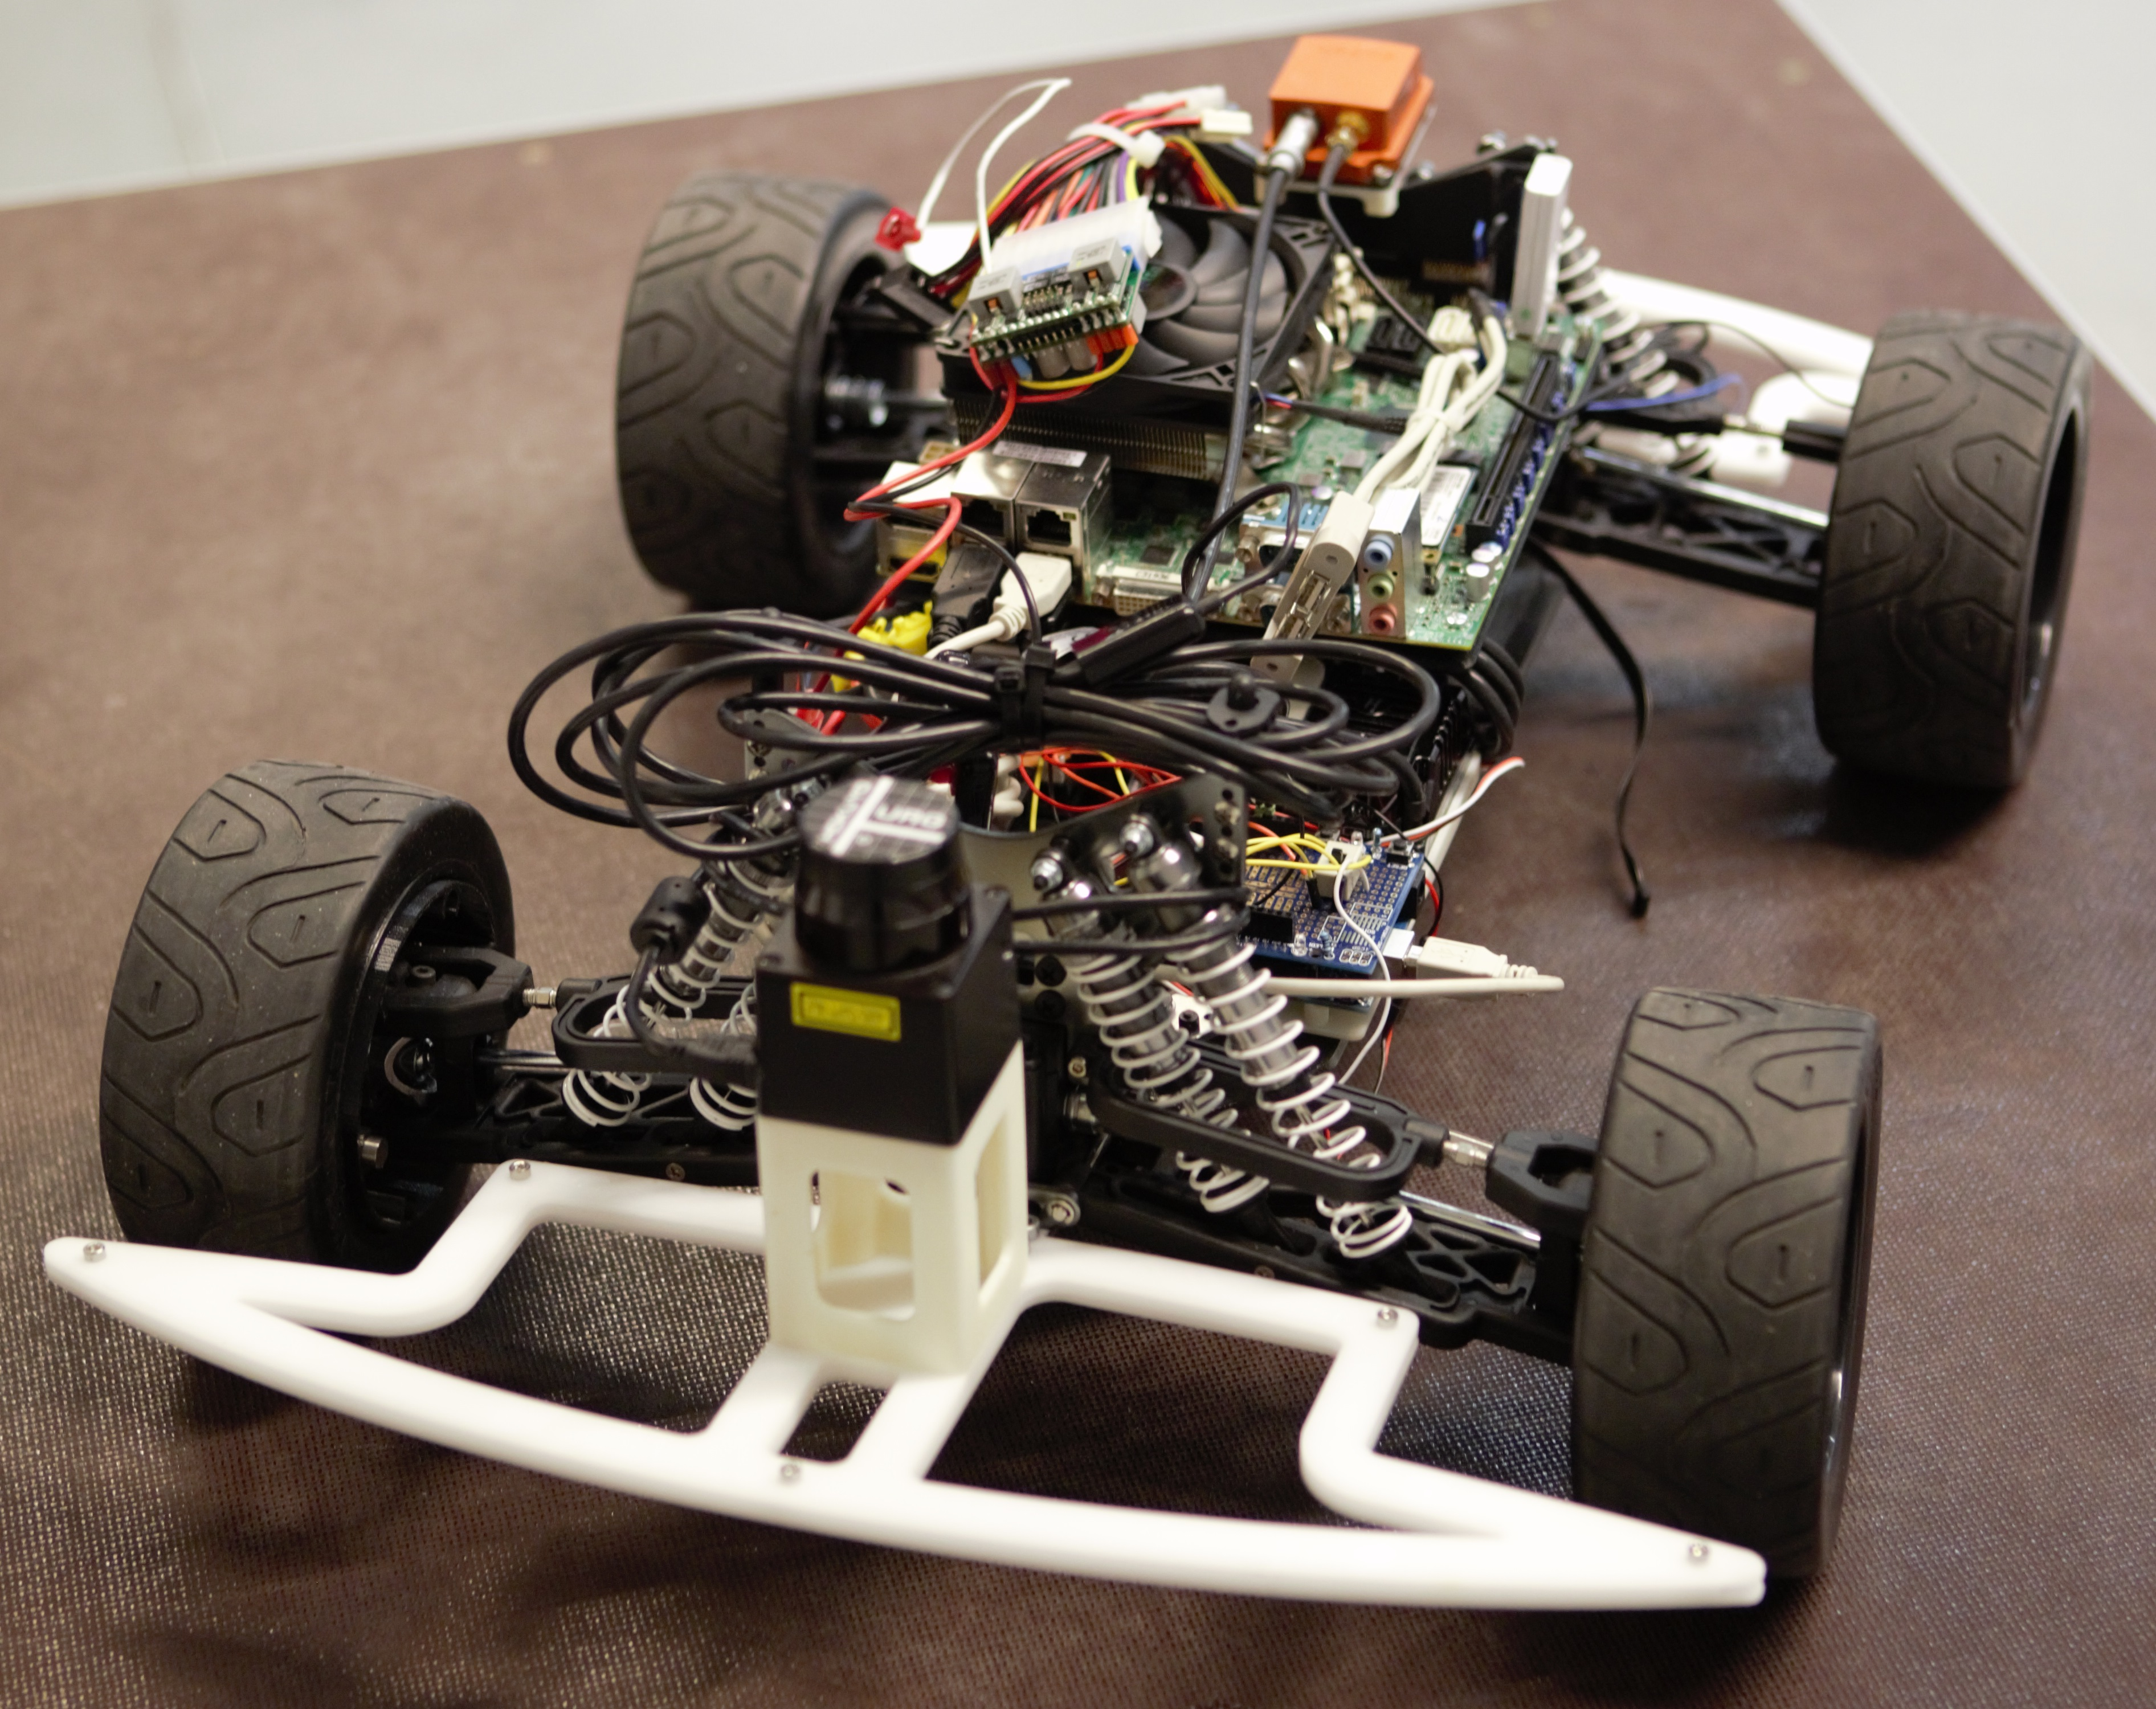
\includegraphics[width=\textwidth]{car}
	\caption{Picture of the rc-car}
	\label{fig:rccar_overview}
\end{figure}


\newpage
%=========================================================================================
\section{Hardware}
%=========================================================================================
\label{sec:overview_hardware}

This section will give a short introduction to the hardware which can be found on the car.

%=========================================================================================
\subsection{Motors and controllers}
\label{sec:overview_motors}

On the car we can find two electrical motors, one for driving the car and one for the steering. 

\begin{figure}[h]
	\centering
		\includegraphics[width=0.5\textwidth]{brushless_motor}
	\caption{HACKER Skalar 8 brushless motor}
	\label{fig:brushless_motor}
\end{figure}


In picture \reffig{brushless_motor} we can see the electrical brushless motor which is used to drive the wheels.The motor is connected to the wheels over a gear and two differentials. Table \reftab{motor_details} gives some details of the used type. More information can be found here:

\hyperref[http://www.hacker-carline.de/produkte/skalar-motoren/hacker-skalar-10/]{http://www.hacker-carline.de/produkte/skalar-motoren/hacker-skalar-10/}

\begin{table}[b]
	\centering	
	\begin{tabular}{cc} % eine Tabelle mit drei Spalten, in denen der Text jeweils zentriert ist
		\hline 
		Name: & HACKER Skalar 8 1750 \\
		max. Power (W): & 1650 \\
		max. RPM (1/min): & 25900 \\
		max. voltage (V): & 14.8 \\
		max. current (A): & 110 \\
		\hline
	\end{tabular}
	\caption{Hacker Skalar 8 - Details} % Die Beschriftung der Tabelle
	\label{tab:motor_details}
\end{table}


For steering, there is a second motor at the front of the car.

Both motors bring its own controllers which take a PWM-signal as input to set the desired revolution rate or angle. The principal is shown in picture \reffig{pwm_signals}. Both input signals are provided by a little Arduino board (see next section 1.1.2).

\begin{figure}[h]
	\centering
		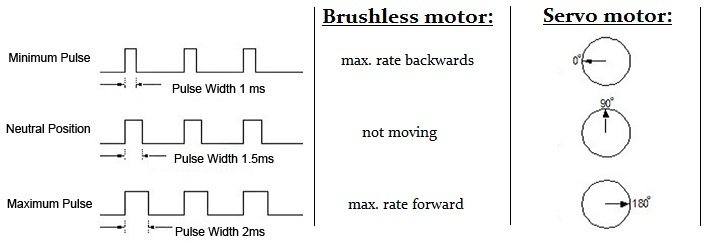
\includegraphics[width=\textwidth]{pwm_signals}
	\caption{PWM-signals for the motors}
	\label{fig:pwm_signals}
\end{figure}


\subsection{Arduino board}
\label{sec:overview_arduino}
\begin{figure}[h]
	\centering
		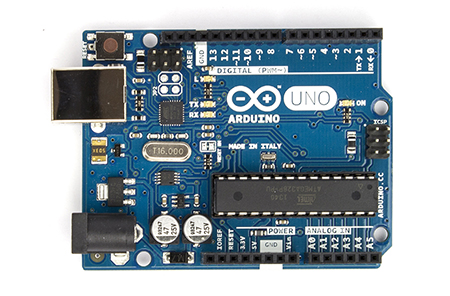
\includegraphics[width=0.35\textwidth]{arduino}
	\caption{Arduino UNO board}
	\label{fig:arduino}
\end{figure}

To provide the signals to the motor controllers there is a little Arduino UNO board on the car which can be seen in picture \reffig{arduino}. It receives the PWM-values from the mainboard of the car via USB and sets them to the output pins which are connected to the controllers.

\subsection{Linux-Board}
\label{sec:overview_board}

For computing there is a Supermicro X10SLV motherboard with a Intel Core i7 processor on it. To control the system we use Ubuntu 14.04 and a special software framework called ROS (see section \refsec{overview_software}). Table \ref{tab:computer_details} gives a short overview of the computer system. More information can be found on:

\hyperref[http://www.supermicro.com/products/motherboard/Core/H81/X10SLV.cfm]{http://www.supermicro.com/products/motherboard/Core/H81/X10SLV.cfm}

\begin{table}[h]
	\centering	
	\begin{tabular}{cc} % eine Tabelle mit drei Spalten, in denen der Text jeweils zentriert ist
		\hline 
		Motherboard: & Supermicro X10SLV \\
		Processor: & Intel Core i7 8 x 3GHz \\
		Memory: & 16GB DDR3 \\
						& 128GB Flash memory \\
		\hline
	\end{tabular}
	\caption{Computer system - Details} % Die Beschriftung der Tabelle
	\label{tab:computer_details}
\end{table}

\newpage
\subsection{Laserscanner}
\label{sec:overview_laserscanner}

\begin{figure}[h]
	\centering
		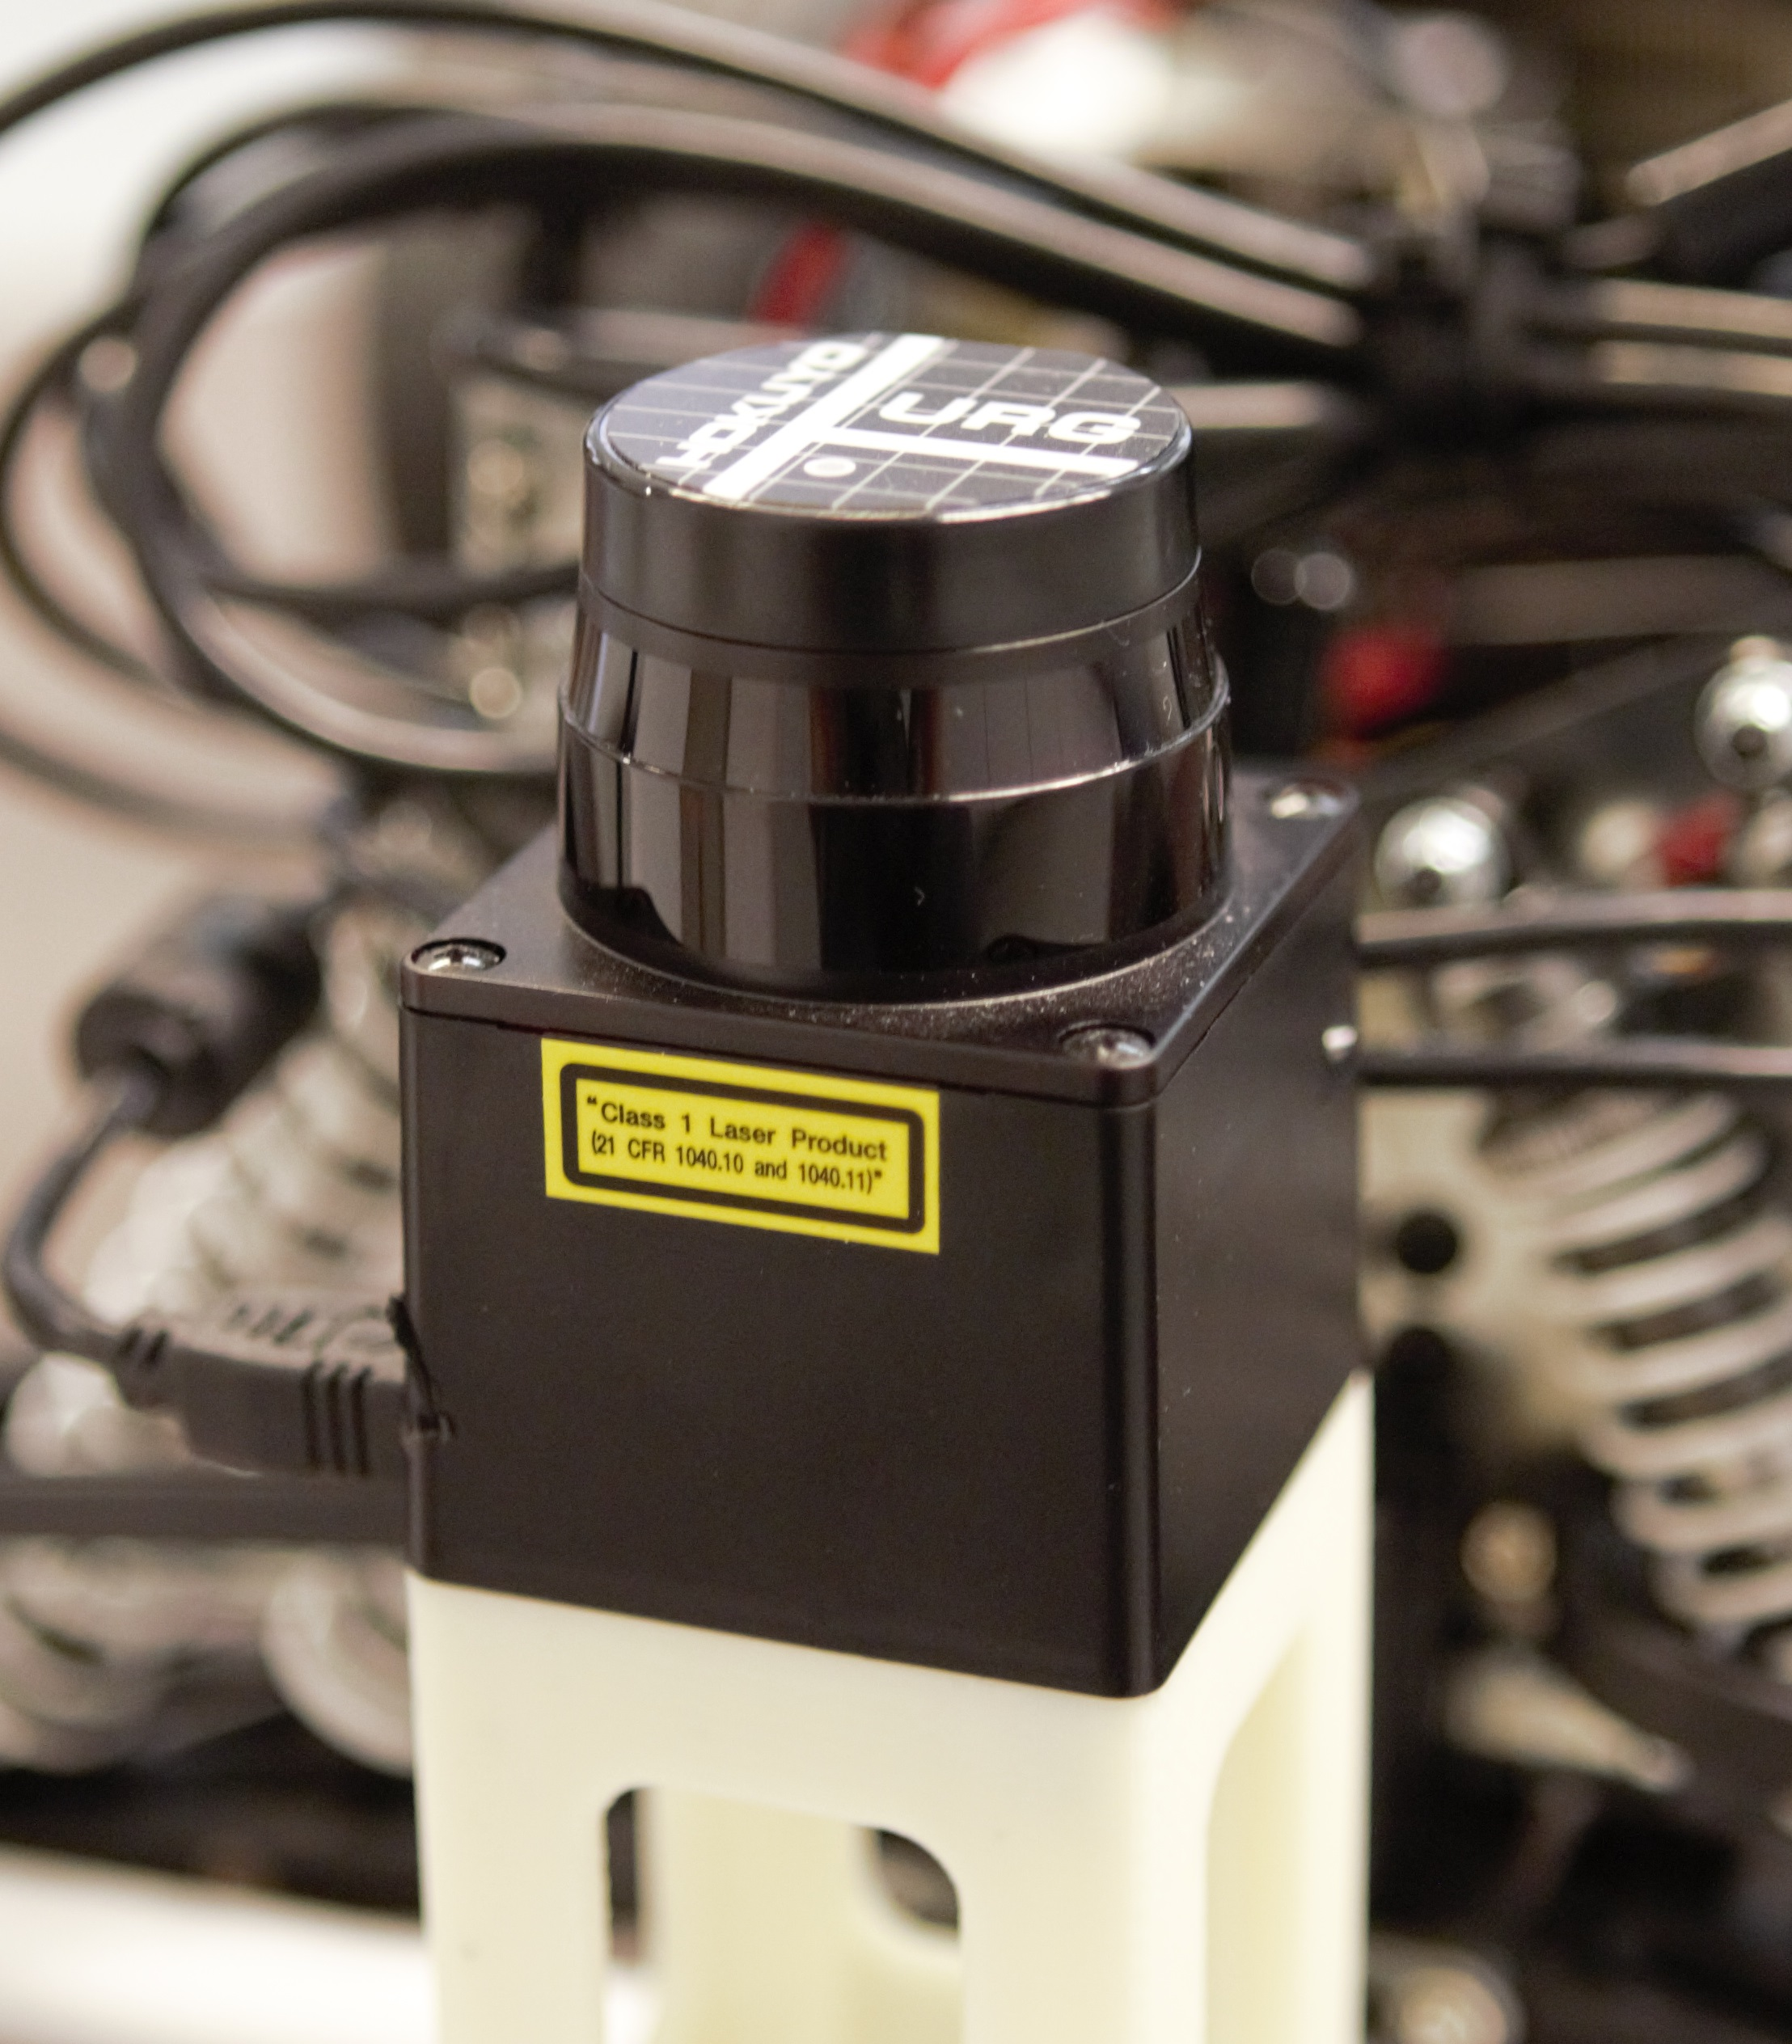
\includegraphics[width=0.35\textwidth]{hokuyo_urg_04lx}
	\caption{Hokuyo URG-04LX-UG01}
	\label{fig:hokuyo}
\end{figure}

At the front of the car we can find a Hokuyo URG-04LX-UG01 laserscanner (see picture \reffig{hokuyo}). The scanner is used for location in a given 2-D map or to create maps while the car is moving through the environment. For detailed information about the scanner refer to:

\hyperref[https://www.hokuyo-aut.jp/02sensor/07scanner/urg_04lx_ug01.html]{https://www.hokuyo-aut.jp/02sensor/07scanner/urg\_04lx\_ug01.html}

\begin{table}[h]
	\centering	
	\begin{tabular}{cc} % eine Tabelle mit drei Spalten, in denen der Text jeweils zentriert ist
		\hline 
		Name: & Hokuyo URG-04LX-UG01 \\
		Measuring area: & 20 to 5600mm(white paper with 70mm×70mm), 240\textdegree \\
		Accuracy: & 60 to 1,000mm : ±30mm, \\
							&	1,000 to 4,095mm : ±3 percent of measurement \\
		Scanning time & 100ms/scan \\
		\hline
	\end{tabular}
	\caption{Laserscanner - Details} %
	\label{tab:laser_details}
\end{table}


\newpage
\subsection{Inertial measurement unit (IMU)}
\label{sec:overview_imu}

\begin{figure}[h]
	\centering
		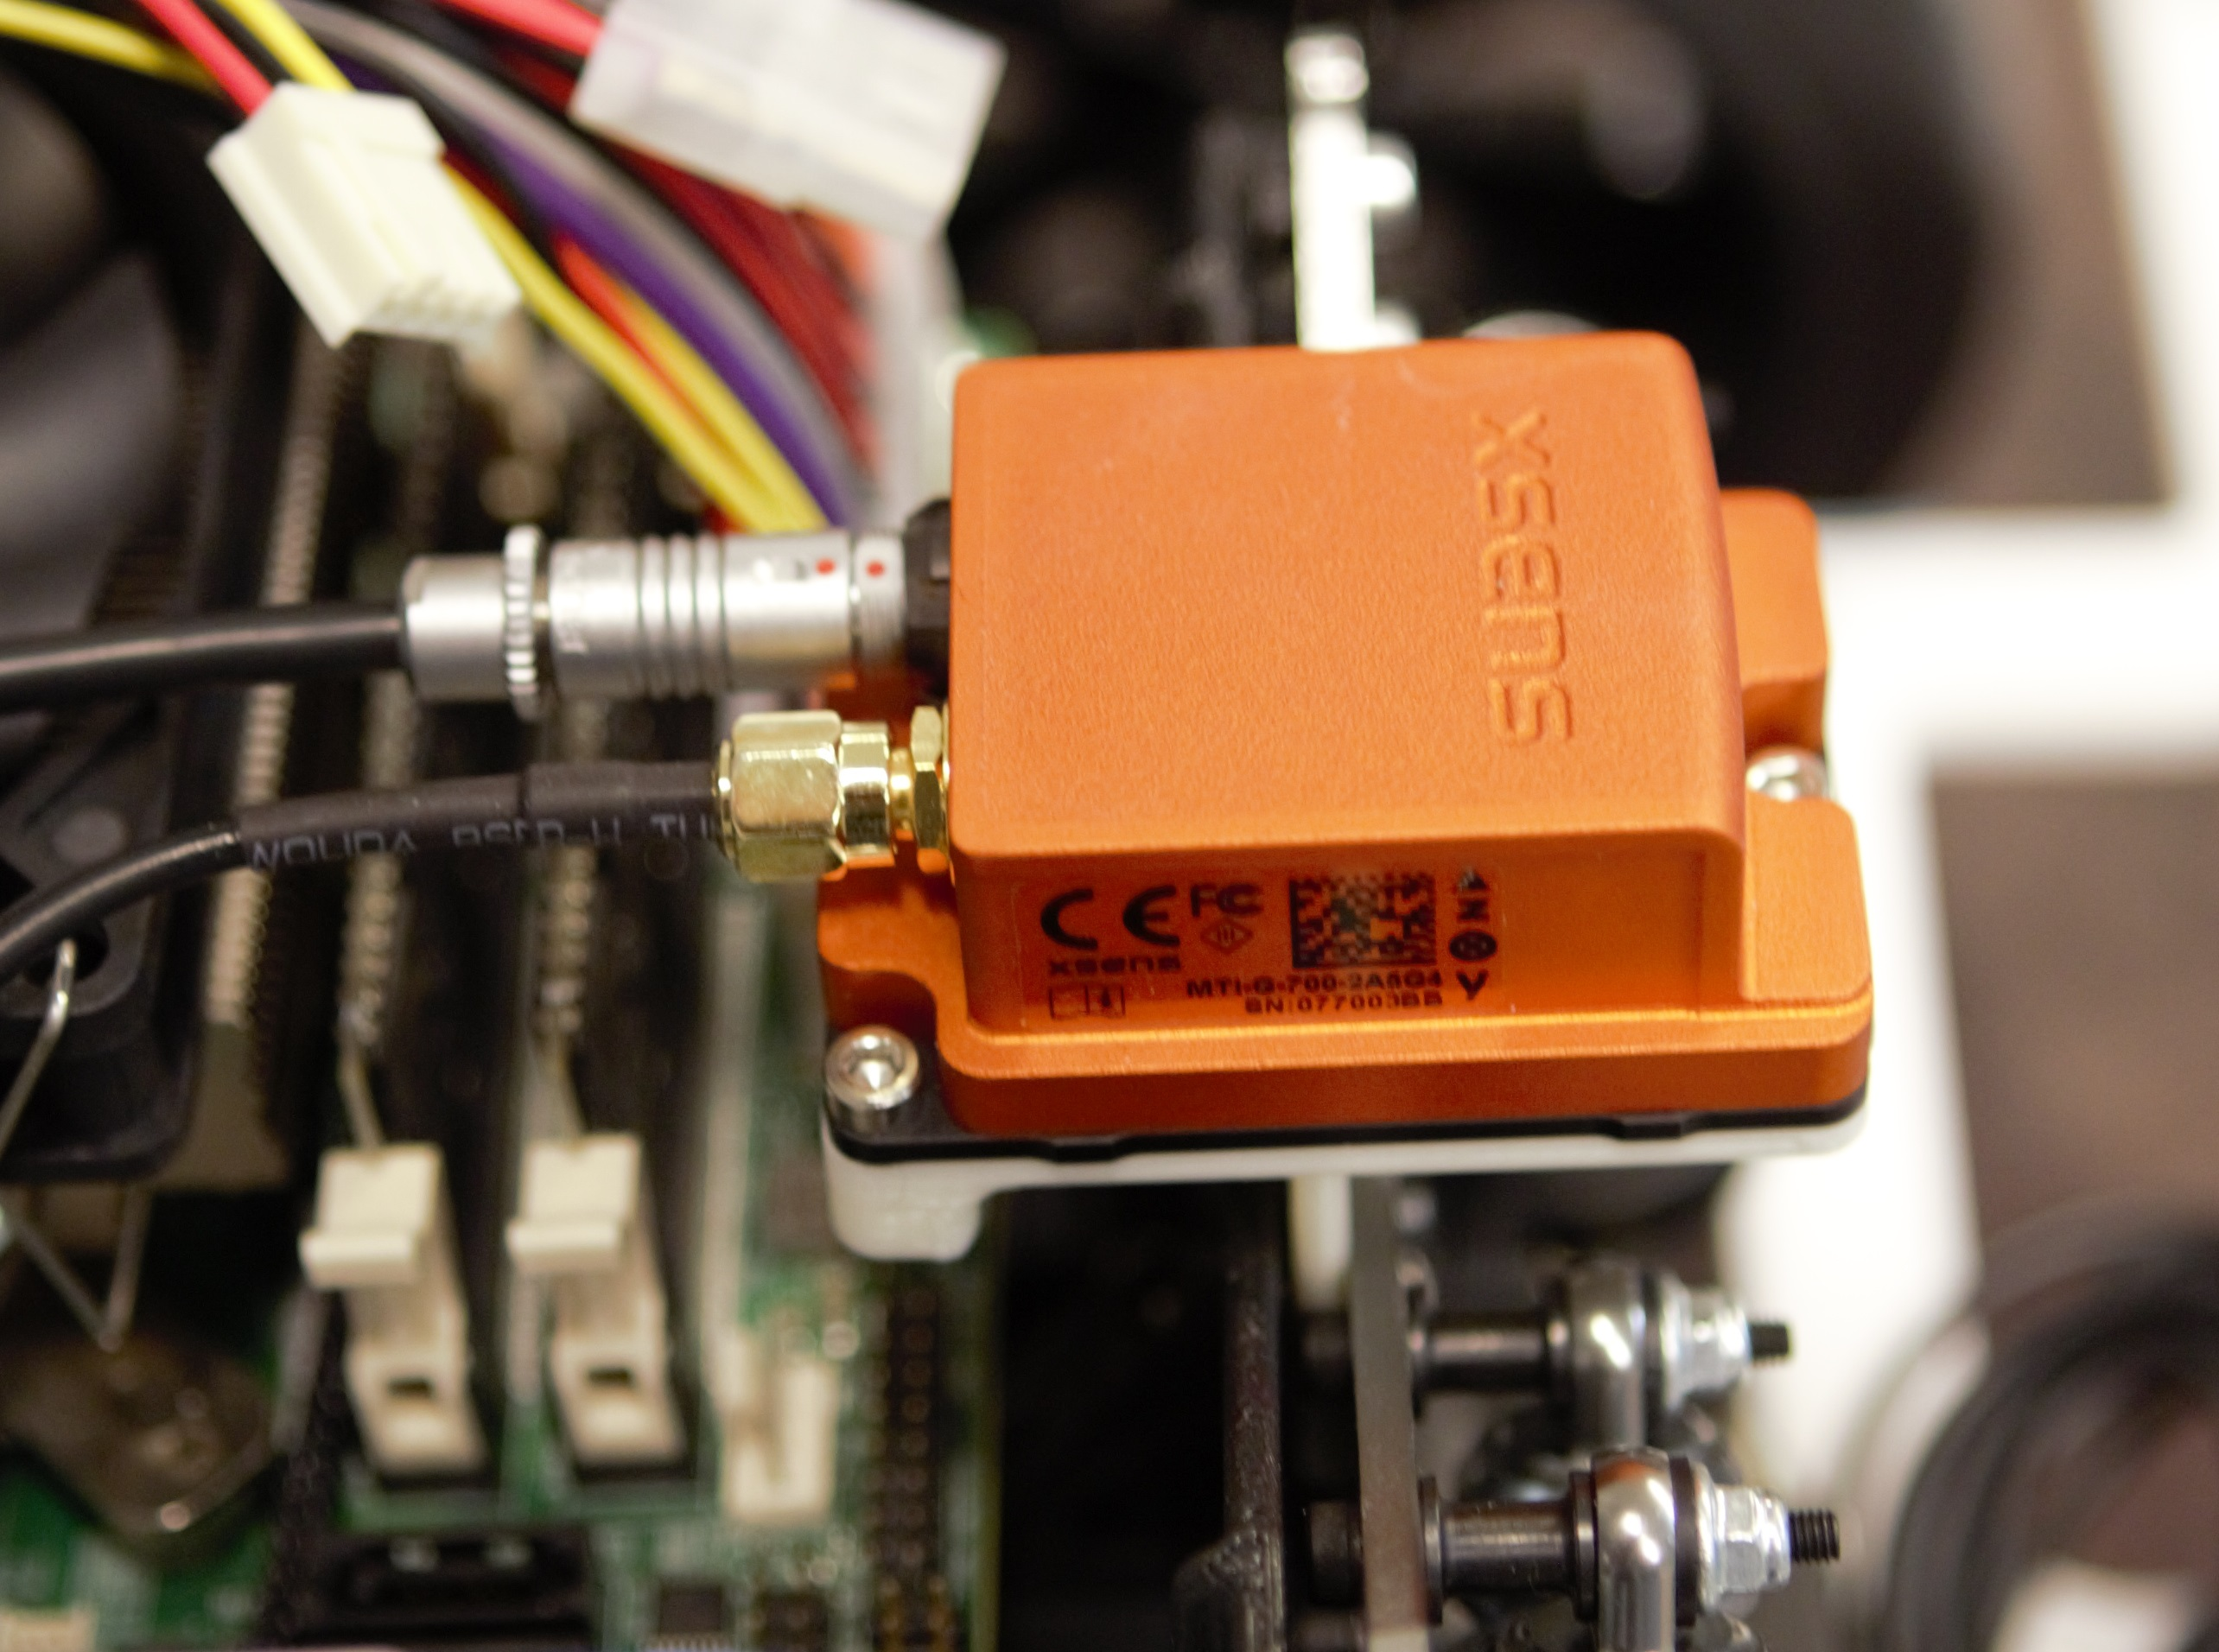
\includegraphics[width=0.4\textwidth]{xsens}
	\caption{XSens MTi-G-700}
	\label{fig:xsens}
\end{figure}

At the back of the car there is an X-Sens MTI-G-700 Inertial Measurement Unit (IMU). It contains sensors for accelerations in every spatial direction, for angle velocities and orientation about each axis and a GPS-module. Table \reftab{imu_details} gives some details of the module. For more information see: 

\hyperref[http://www.xsens.com/products/mti-g-700/]{http://www.xsens.com/products/mti-g-700/}

\begin{table}[h]
	\centering	
	\begin{tabular}{cc} % eine Tabelle mit drei Spalten, in denen der Text jeweils zentriert ist
		\hline 
		Name: & XSens MTi-G-700 \\
		Output frequency: & Up to 2000Hz \\
		Standard full range gyro: & 450 \textdegree/s \\
		Standard full range acc		& 50 m/s2 \\
		In-run bias stability gyro& 10 \textdegree/h \\
		\hline
	\end{tabular}
	\caption{IMU - Details} % Die Beschriftung der Tabelle
	\label{tab:imu_details}
\end{table}




%=========================================================================================
\section{Software}
%=========================================================================================
\label{sec:overview_software}

The operating system currently running on the linux board of the car is Ubuntu 14.04. To work with the hardware there is installed a software framework called Robot Operating System (ROS) which provides a big number of libraries and tools to work with robots. On the car we use the currently newest version: ROS Indigo \footnote{Since ROS Fuerte there are two different build systems. We use the catkin build system}. 

 At the beginning of the course you should get familiar with the functionality of ROS. A good start are the official tutorials on: 

\hyperref[http://wiki.ros.org/]{http://wiki.ros.org/}

After working with the tutorials you should understand the concept of nodes and topics and be able to create and build your own package. To work with the car there is a package on GitHub you can download and install on your system. See the next chapter for more information.


%=========================================================================================




%
% Beispielkapitel: Bedienung dieser Vorlage
%

% Zum Setzen von TeX-Quellcode, der nicht interpretiert werden soll
\newcommand{\makro}[1]{\texttt{\textbackslash{}#1\{\}}}

\chapter{Set up the hardware}
\label{sec:setup}

The following chapter will show you how to connect the car to different power supplies.There are two possibilities to power the car electrically:

\begin{itemize}
		\item Power from battery:\\
					Of course the whole car can be powered by battery to drive it around wireless.
		\item External power source: \\
					The Linux Board can also be powered by an external power source for long programming and debugging sessions. This avoids data loss in case of an empty battery. If only the board is supplied and the brushless motor is disconnected from the power supply the battery will last for about one hour.					
\end{itemize}



\begin{wrapfigure}[15]{l}{0.35\textwidth}
  \begin{center}
    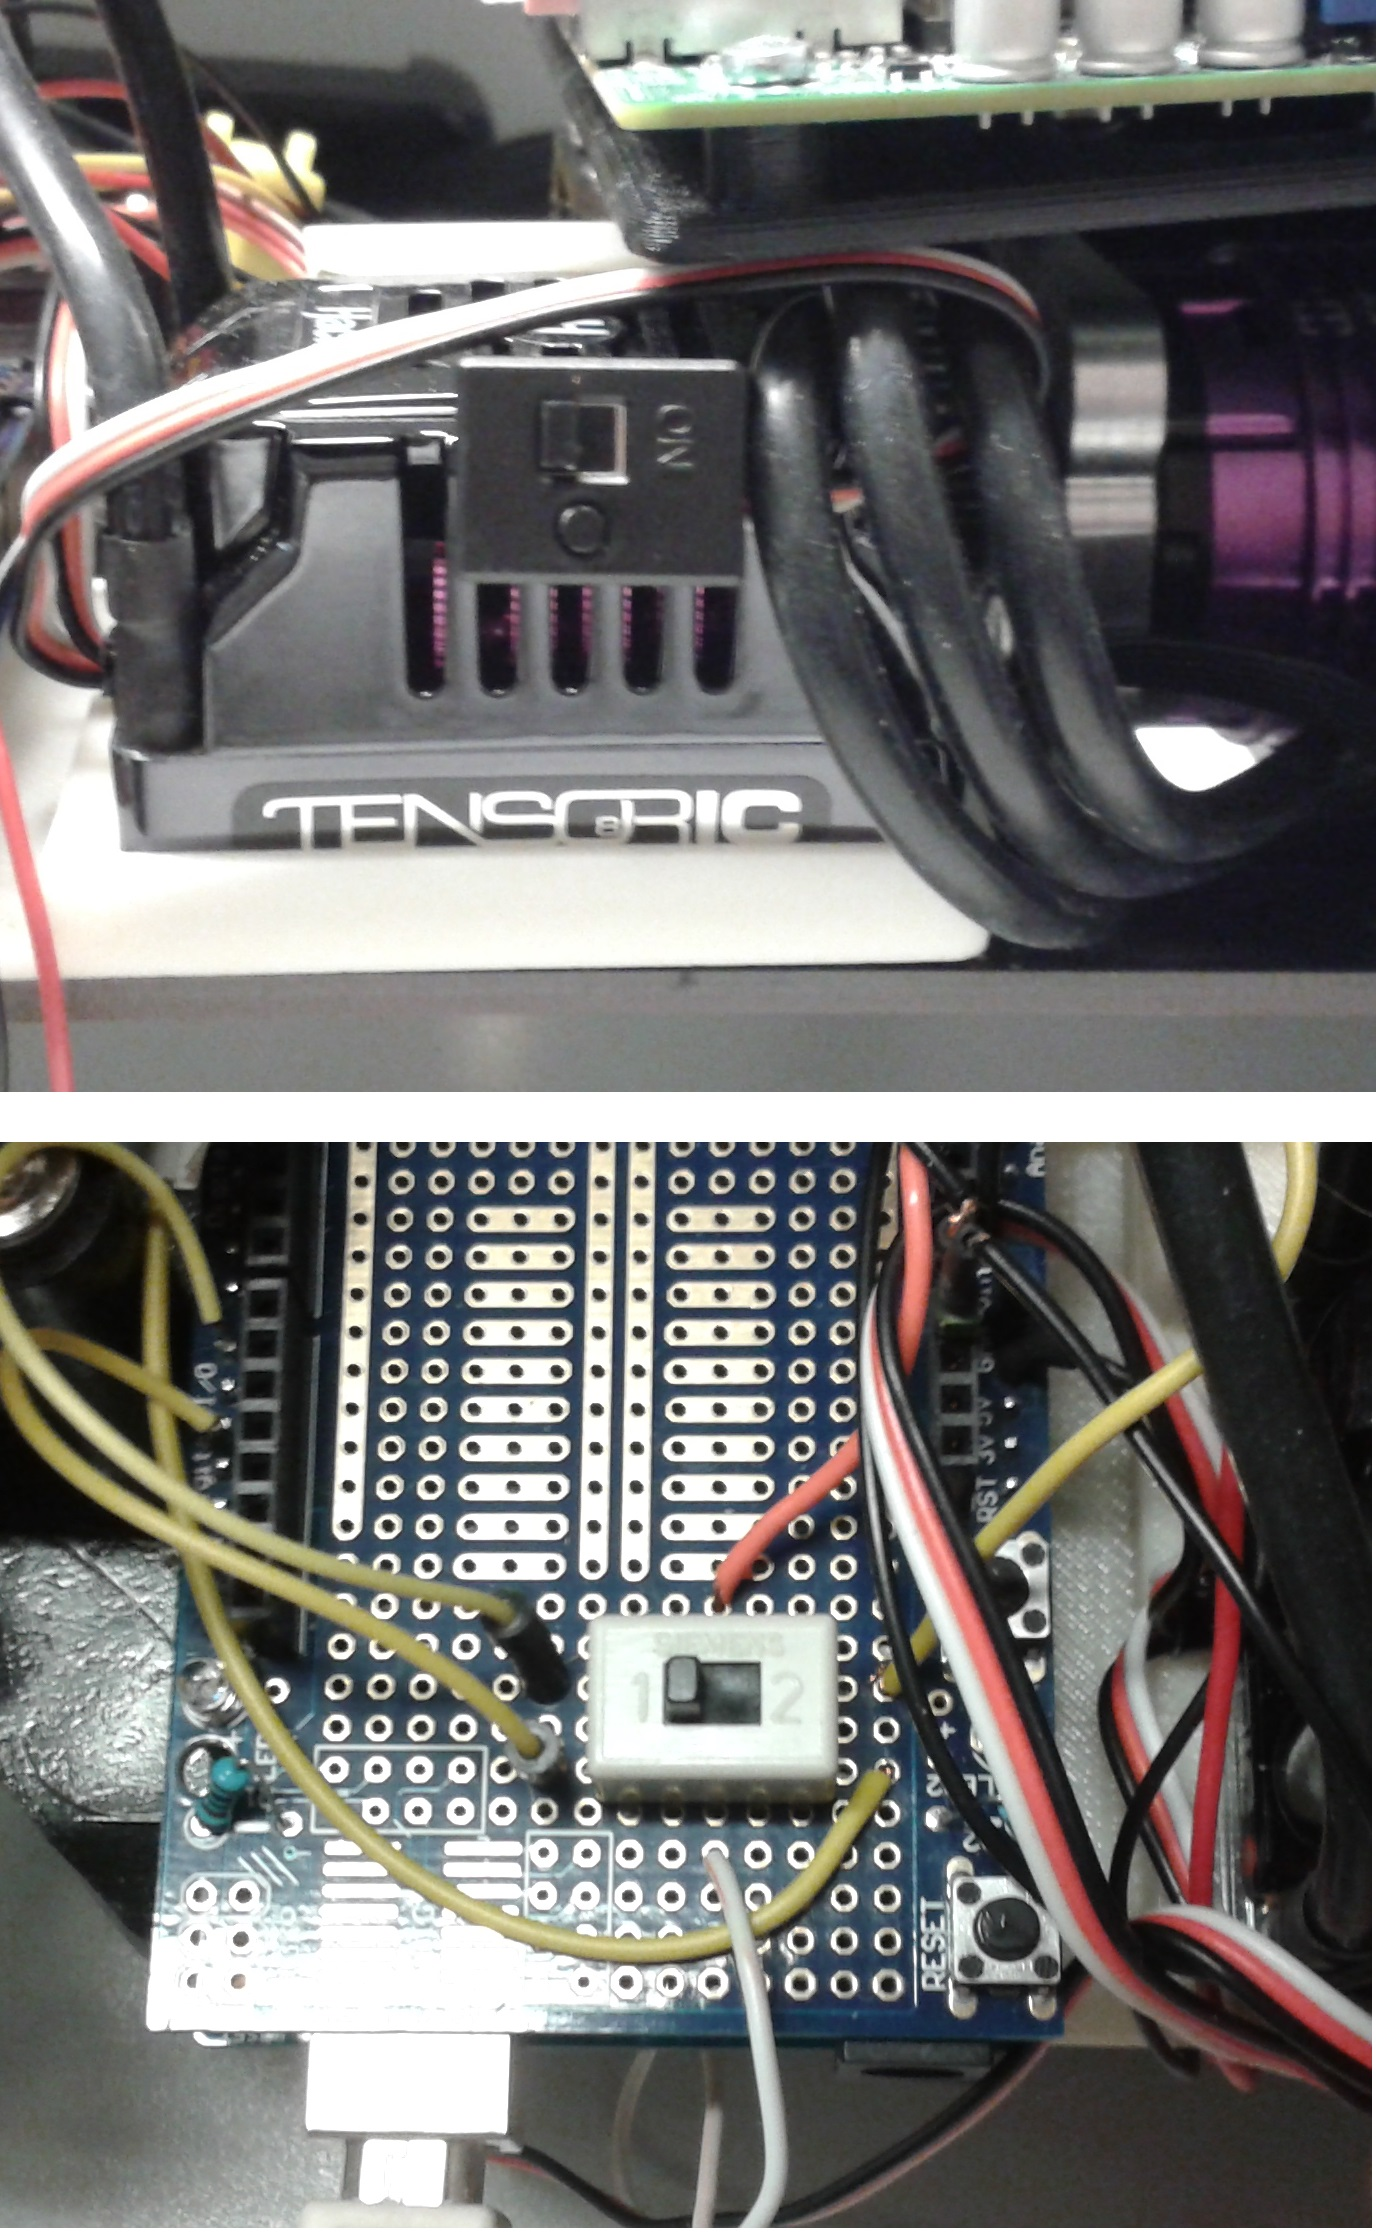
\includegraphics[width=0.33\textwidth]{switches}
		\caption{Switches for brushless motor}
		\label{fig:switches}
  \end{center}	
\end{wrapfigure} 

Power supply for the brushless motor can disconnected by a switch, which you can see in picture \reffig{switches} on the top. With the switch shown on the bottom you can select the source of the input signals for the brushless motor controller:

\begin{itemize}
\item Position 1:\\
In this position the input signal is taken from the arduino, which receives it from the ROS \texttt{/servo} topic.
\item Position 2:\\
In this positon the input signal is taken directly from the receiver for the original remote controller. This receiver is connected directly to the brushless controller. It is not connected to the Arduino or the Linux-Board in any way.
\end{itemize}



\newpage

\section{Power from external power source}
\label{setup_external}

\begin{figure}[h]
	\centering
		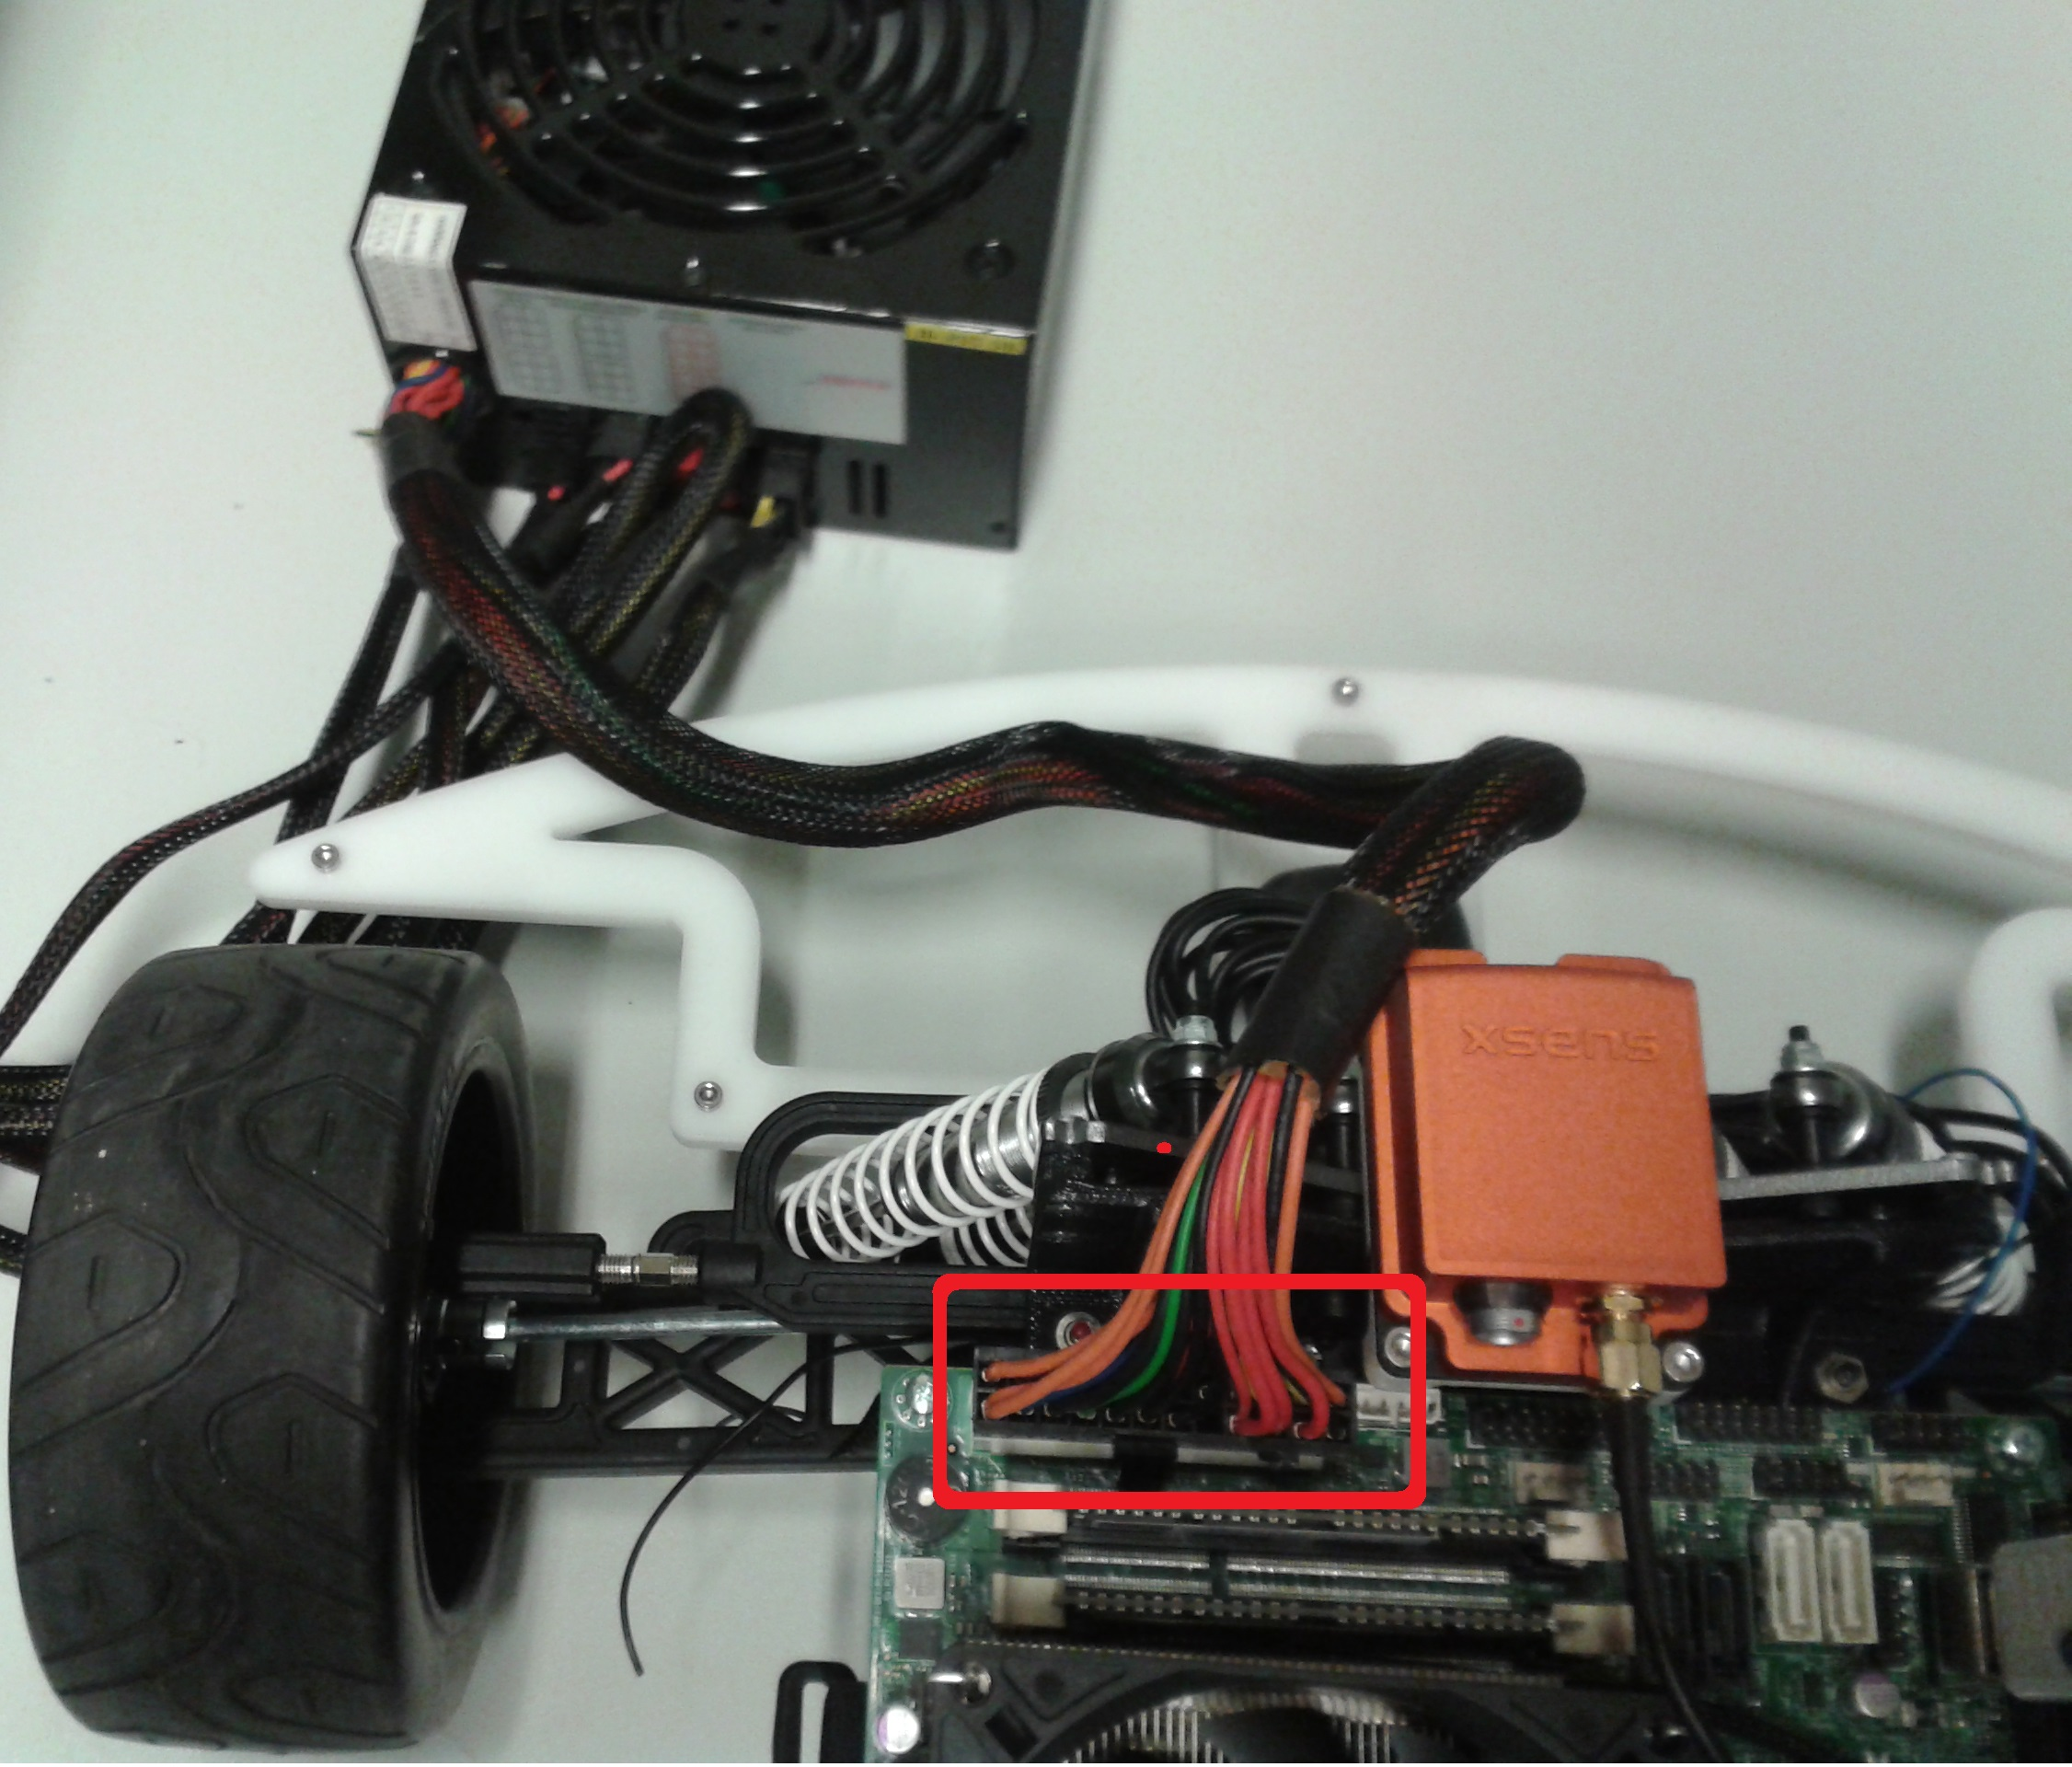
\includegraphics[width=0.55\textwidth]{ext_power}
	\caption{Connection to the external power source}
	\label{fig:ext_power}
\end{figure}
To power the board externally just connect the large 24-pin connector like it is show in picture \reffig{ext_power}. Pay attention: This will not supply the motors. These can only be powered by the battery.

\section{Power from battery}
\label{setup_battery}

\begin{figure}[h]
	\centering
		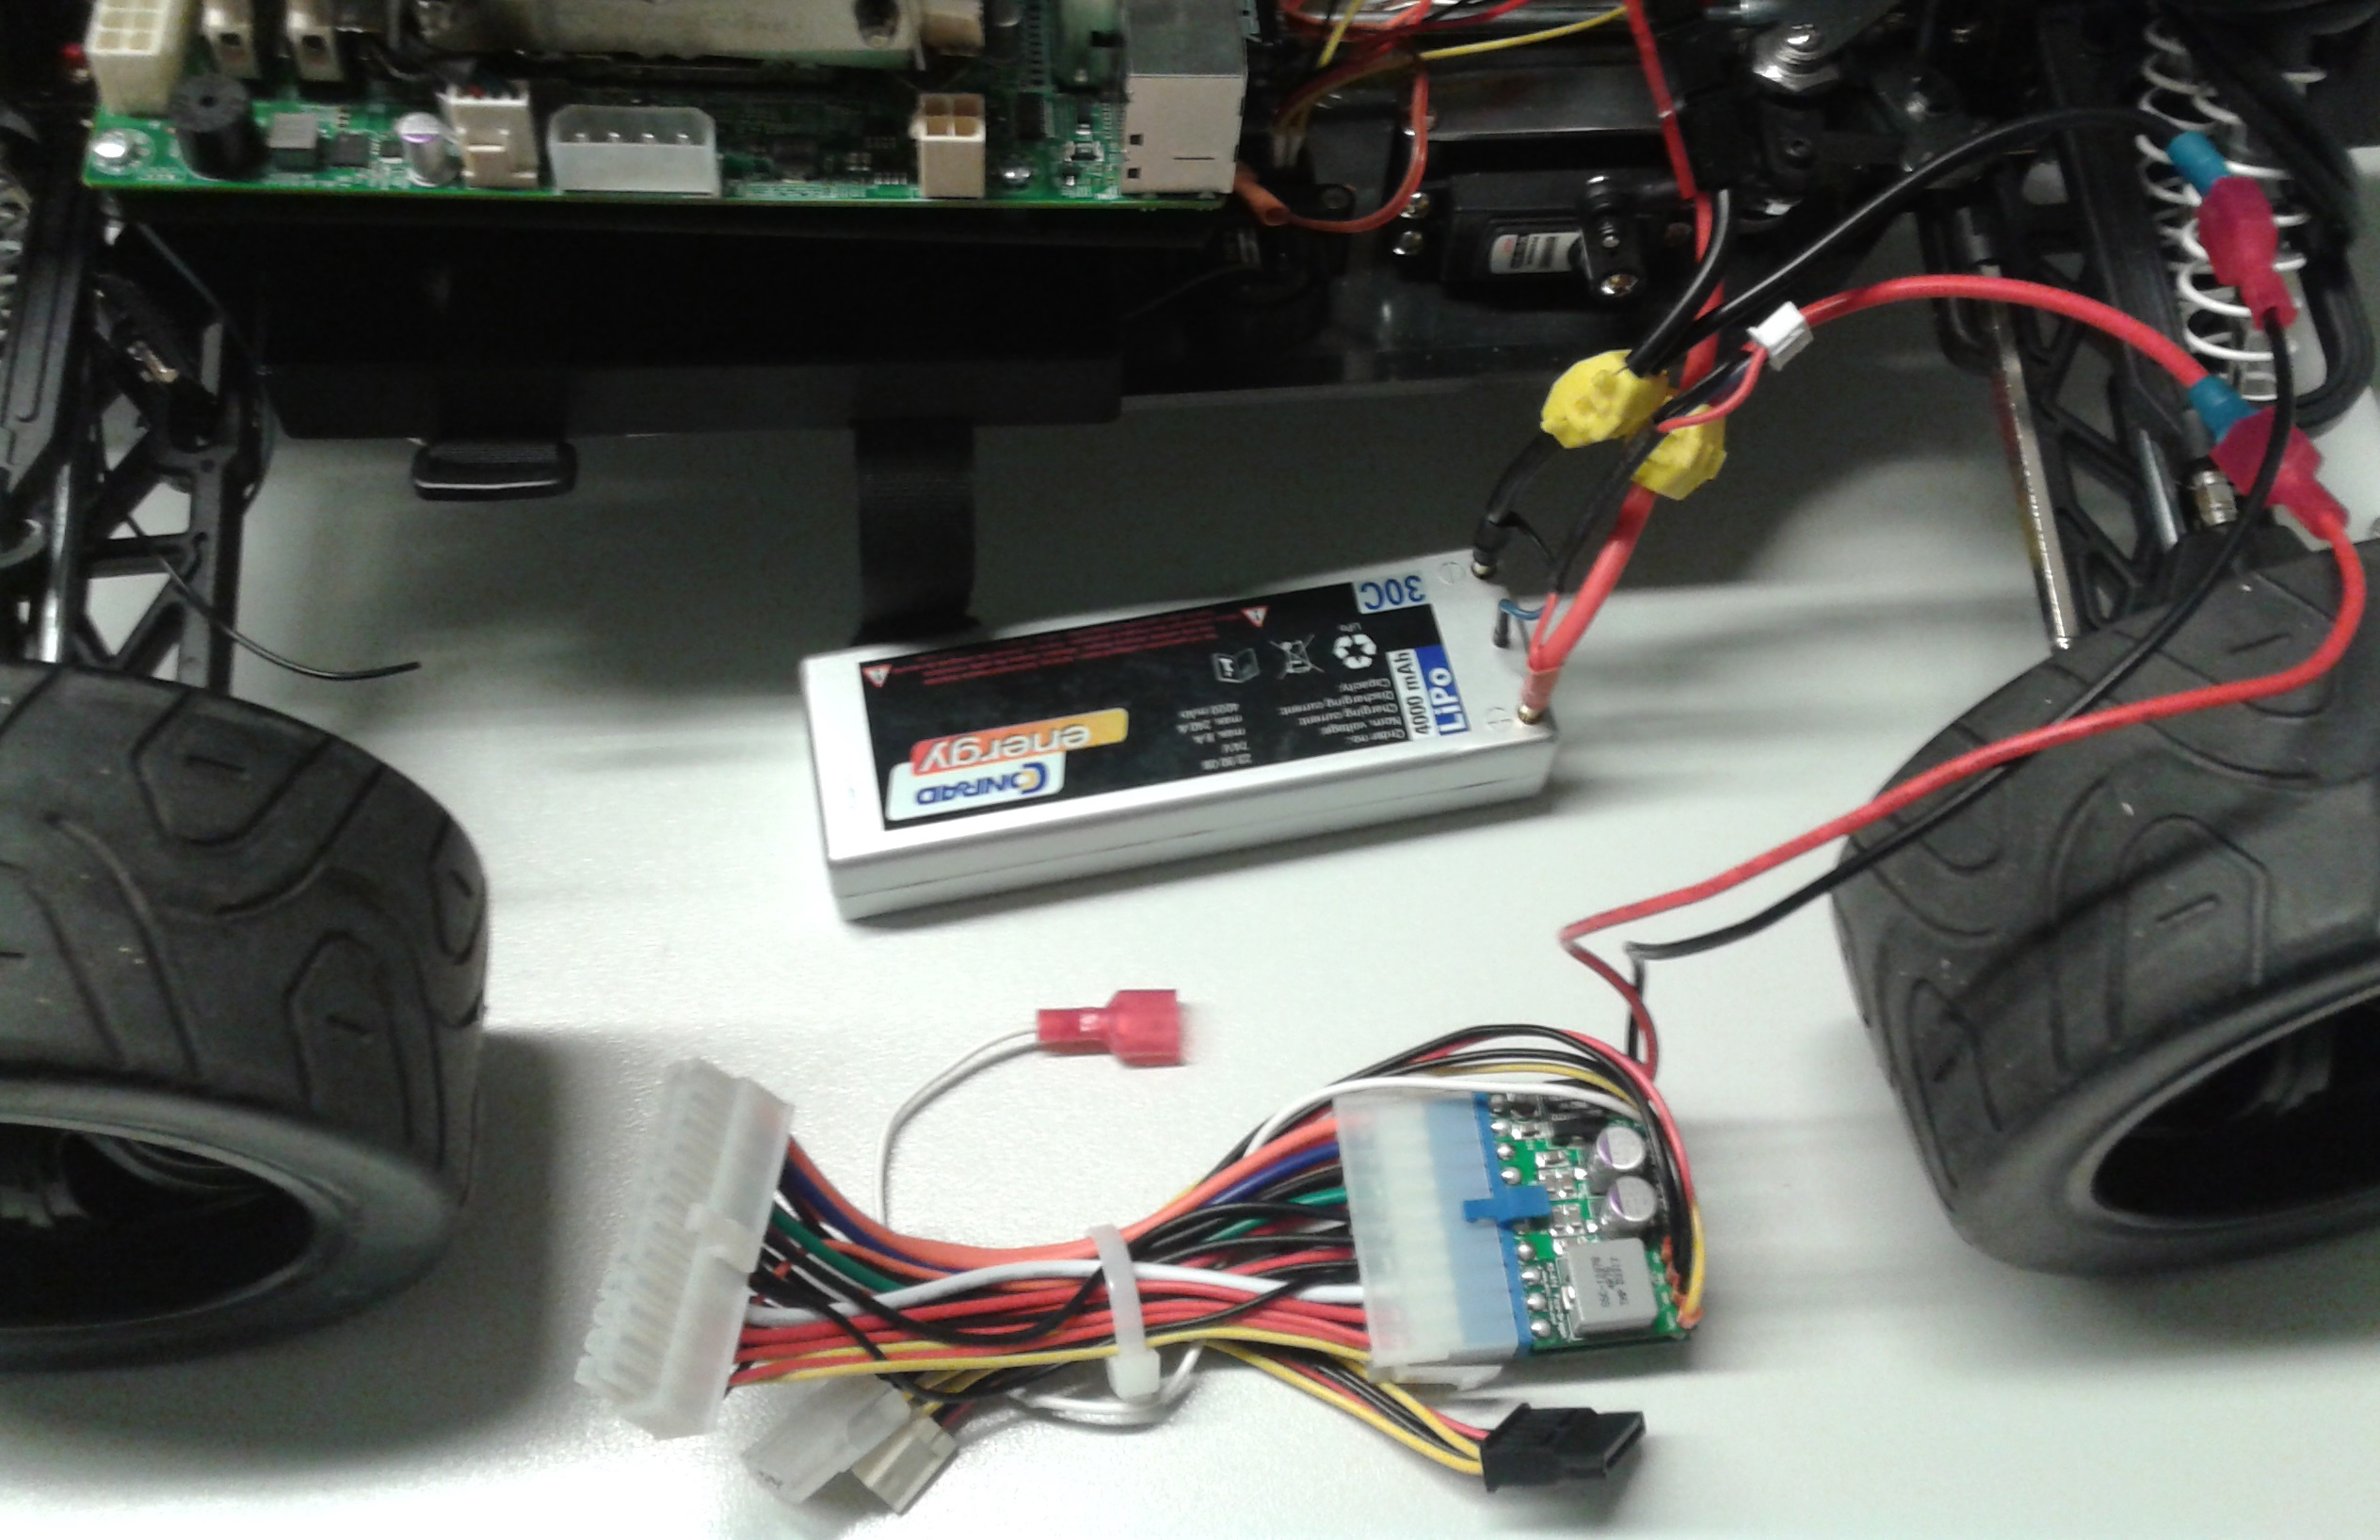
\includegraphics[width=0.55\textwidth]{batt_power}
	\caption{Connection to battery}
	\label{fig:batt_power}
\end{figure}
To supply the board from battery, there is a 12V DC-DC Converter which you can see in picture \reffig{batt_power} obove. Just connect the battery and the converter like in the picture and the plug the 24-pin connector into the board.




% Zum Setzen von TeX-Quellcode, der nicht interpretiert werden soll
\newcommand{\makro}[1]{\texttt{\textbackslash{}#1\{\}}}

\chapter{The TAS-package}
\label{sec:tas_package}

This chapter will show you how to install the TAS-package and get the car running step-by-step. It will give you a short desription of each of the different components. The package contains several self-written nodes and launchfiles to run the hardware (Laserscanner, IMU, Arduino) and the so called Navigation Stack properly on the car. The Navigation Stack provides tools for high level tasks like path planning and localization. The TAS-package also brings some shell scripts, for example to set up the ROS environment correctly. The folder structure can be seen in picture \reffig{tas_folder_struct}.

Most of the files we need in this tutorial are found in the folder \texttt{tas/launch}.

\begin{figure}[htbp]
	\centering
		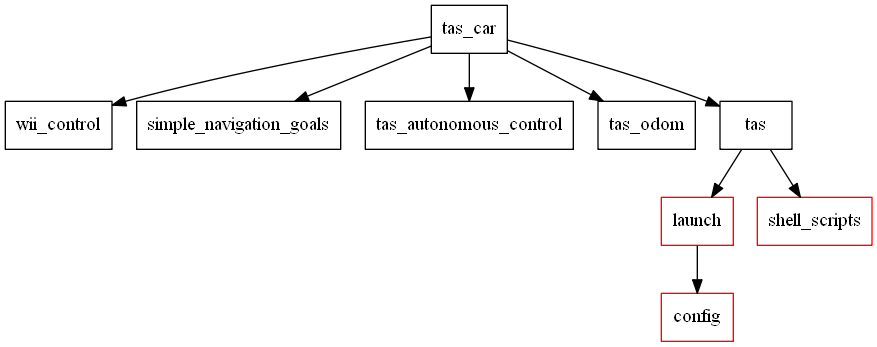
\includegraphics[width=\textwidth]{diagrams/tas_folder_struct}
	\caption{Folder structure of the TAS-package}
	\label{fig:tas_folder_struct}
\end{figure}

\newpage
\section{Installing the TAS-package}
\label{sec:tas_package_install 

As it was mentioned in the previous chapter the TAS-package can be found on GitHub. To install it open a terminal and switch to your catkin workspace directory. In this example we assume your working directory in \texttt{\textasciitilde/catkin\_ws}. To get and build the package on your car type in:

\shellcmd{cd \textasciitilde/catkin\_ws/src}\\
\shellcmd{git clone https://github.com/LSR-TAS/tas\_car}\\

To get the package running there are some preperations needed. Switch to the \texttt{shell\_scripts} folder and run the \texttt{ros\_setup.sh} script:

\shellcmd{cd \textasciitilde/catkin\_ws/src/tas\_car/tas/shell\_scripts}\\
\shellcmd{./ros\_setup.sh}\\

The script will take the following effects:

\begin{itemize}
\item Set rules for USB devices :\\
Usually Ubuntu names and numerates USB devices in a specific way. The numeration depends on the order in which the devices are plugged in. The script applies some rules to the system to assign clear names to the laserscanners and the arduino board.
\item Set up ROS environment:\\
Before working with ROS command line tools it is necessary to source a specific file. The script adds this command to the \texttt{~/.bashrc} file, which is executed each time you open a terminal. Therefore it is not required anymore to type in this command by hand. 
\end{itemize}

\textbf{After running the script, it is necessary to reboot the system.}

When the system has restarted it is ready to build the package. Open a terminal, switch to your catkin workspace and type:

\shellcmd{cd \textasciitilde/catkin\_ws}\\
\shellcmd{catkin\_make}\\

The package manager will now compile and build the code. If there occured no errors during the process the car is now ready to run! Before going on with the next section, please \textbf{reopen the terminal once}.

\newpage
\section{Hardware drivers}
\label{sec:tas_package_drivers}
The follwing section will show you how to run the hardware drivers on the car. After launching them it is already possible to drive the car around and control it manually with the wii controller.

\begin{figure}[h]
	\centering
		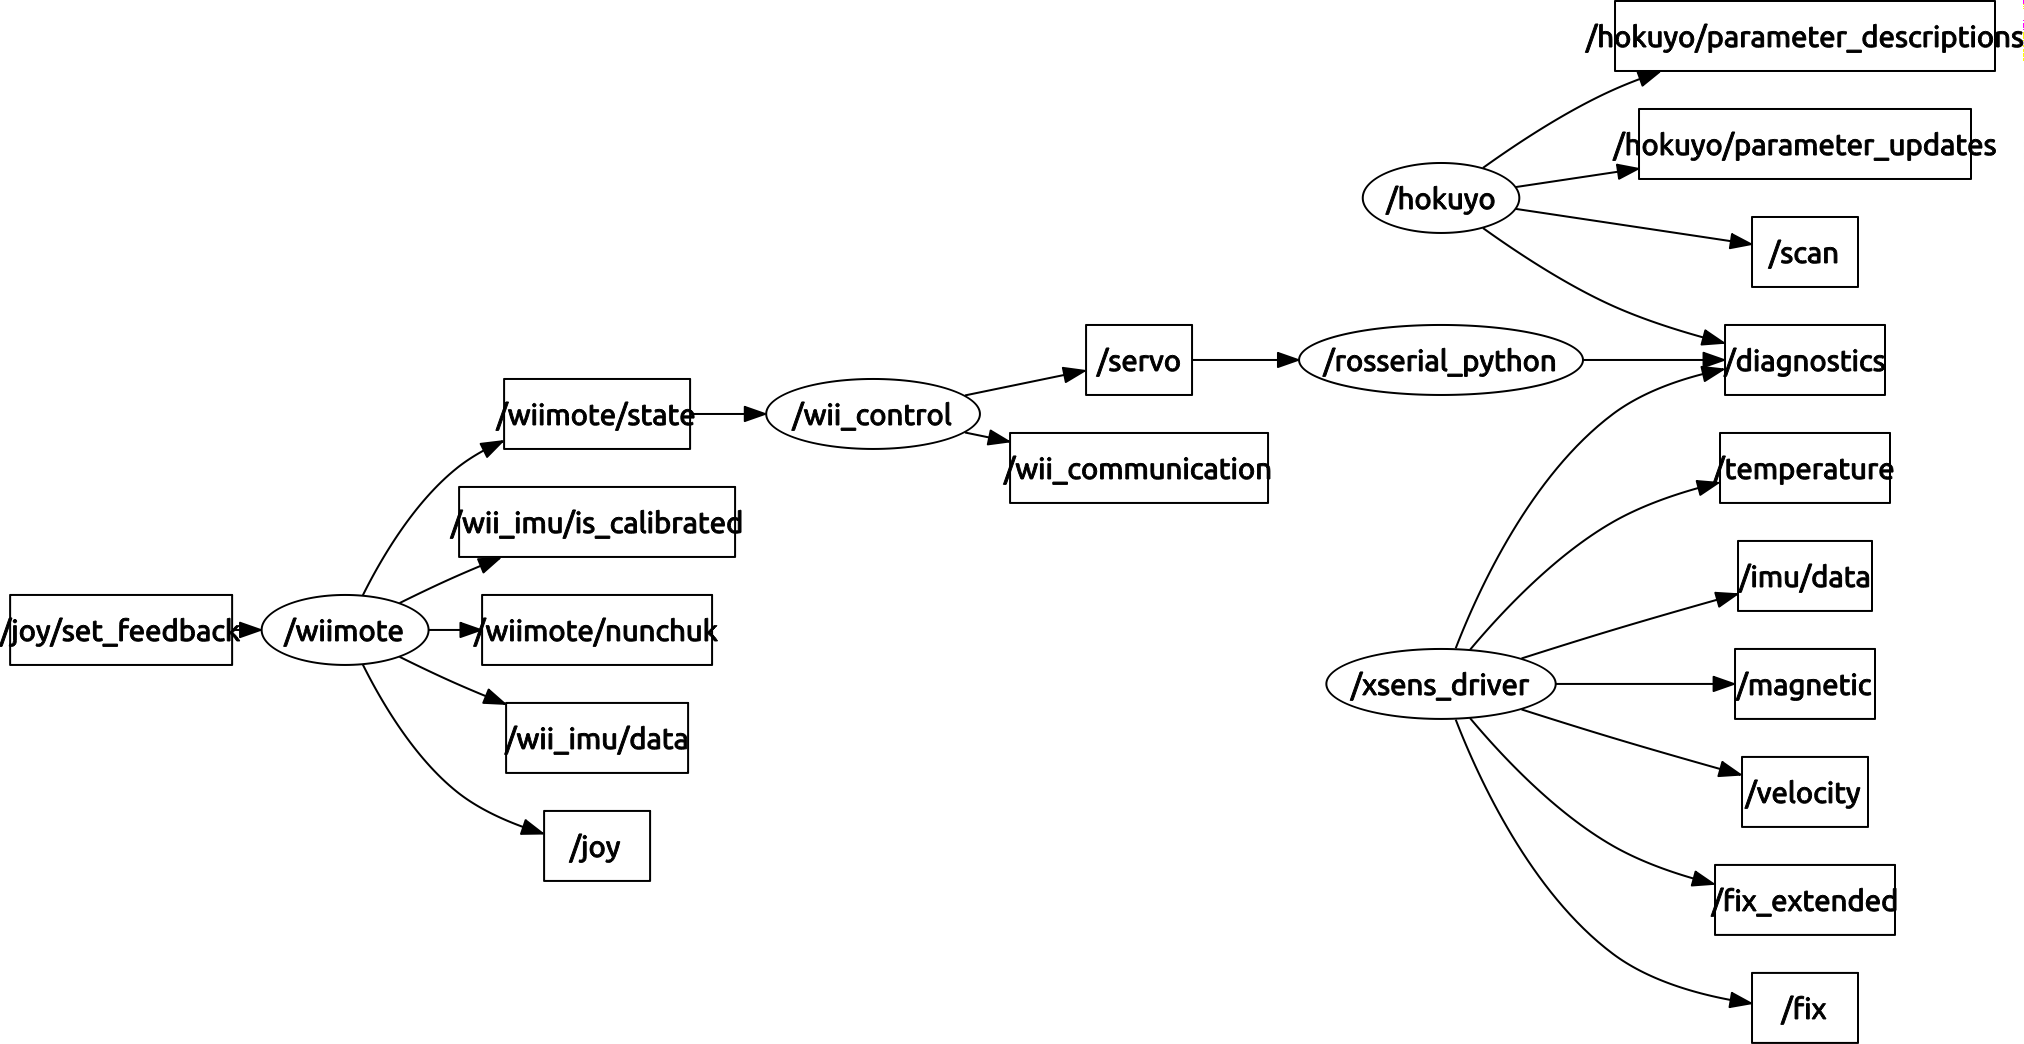
\includegraphics[width=0.9\textwidth]{diagrams/rqt_hardware}
	\caption{ROS nodes for the hardware}
	\label{fig:rqt_hardware}
\end{figure}

\begin{wrapfigure}{r}{0.13\textwidth}
  \begin{center}
    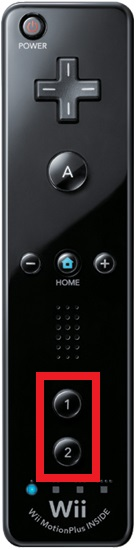
\includegraphics[width=0.13\textwidth]{wii}
		\caption{}
		\label{fig:wii_controller}
  \end{center}	
\end{wrapfigure}

To launch the hardware drivers open a terminal and type in:

\shellcmd{roscd tas/launch}\\
\shellcmd{roslaunch hardware.launch}

This will run several nodes to communicate with the hardware which will be explained in detail in the following sections. To establish the connection to the wii-controller press the the two two buttons at the bottom of the controller (see picture \reffig{wii_controller} on the right) for about 5 seconds until you see a notification in the terminal window. \textbf{If the motors are powered (see section \refsec{setup}), the car is now ready to run!}

In picture \reffig{rqt_hardware} you can see a graphical overview of the running nodes and topics. If you open a terminal and type in:

\shellcmd{rosrun rqt\_graph rqt\_graph}

you should get the same picture.


\subsection{wiimote}
\label{sec:tas_package_drivers_wiimote}
The \texttt{wiimote} node establishes a bluetooth connection to the wii-controller. It reads the inputs from the sticks and buttons of the controller and publishes these information to several ROS topics. Like you certainly have noticed, we use this data as control inputs for the car in manual mode. See the following link for a more detailed description:

\hyperref[http://wiki.ros.org/wiimote?distro=indigo]{http://wiki.ros.org/wiimote?distro=indigo}

\subsection{wii\_control}
\label{sec:tas_package_drivers_wii_control}
The motor controllers require a special PWM signal as control inputs (see picture \reffig{pwm_signals}). The \texttt{wii\_control} node takes the inputs from the wii-controller, calculates the corresponding PWM values and publises them to the \texttt{/servo} topic.


\subsection{rosserial\_python}
\label{sec:tas_package_drivers_rosserial}
The \texttt{rosserial\_python} node takes the PWM values from the \texttt{/servo} topic and sends them to the arduino via the USB port. It mainly implements the communication channel between nodes and topics over a (virtual) serial port. For correct communication there has to be installed the so called \texttt{rosserial\_client} on the arduino. For more information refer to:

\hyperref[http://wiki.ros.org/rosserial]{http://wiki.ros.org/rosserial}

\subsection{hokuyo\_node}
\label{sec:tas_package_drivers_hokuyo}
The \texttt{hokuyo\_node} is the driver for the laserscanner. It reads the measured data from the scanner via USB and publishes the to the \texttt{/scan} topic.

\hyperref[http://wiki.ros.org/hokuyo_node]{http://wiki.ros.org/hokuyo\_node}

\subsection{xsens\_driver}
\label{sec:tas_package_drivers_xsens}

The package provides a driver for several different IMUs from the XSens company. It reads data from the sensor via USB and publishes it to the \texttt{/imu/data} topic just like the \texttt{hokuyo\_node} does with the laser data.

\hyperref[http://wiki.ros.org/xsens_driver]{http://wiki.ros.org/xsens\_driver}

\newpage
\section{TAS-Odometry}
\label{sec:tas_package_odom}

\begin{figure}[h]
	\centering
		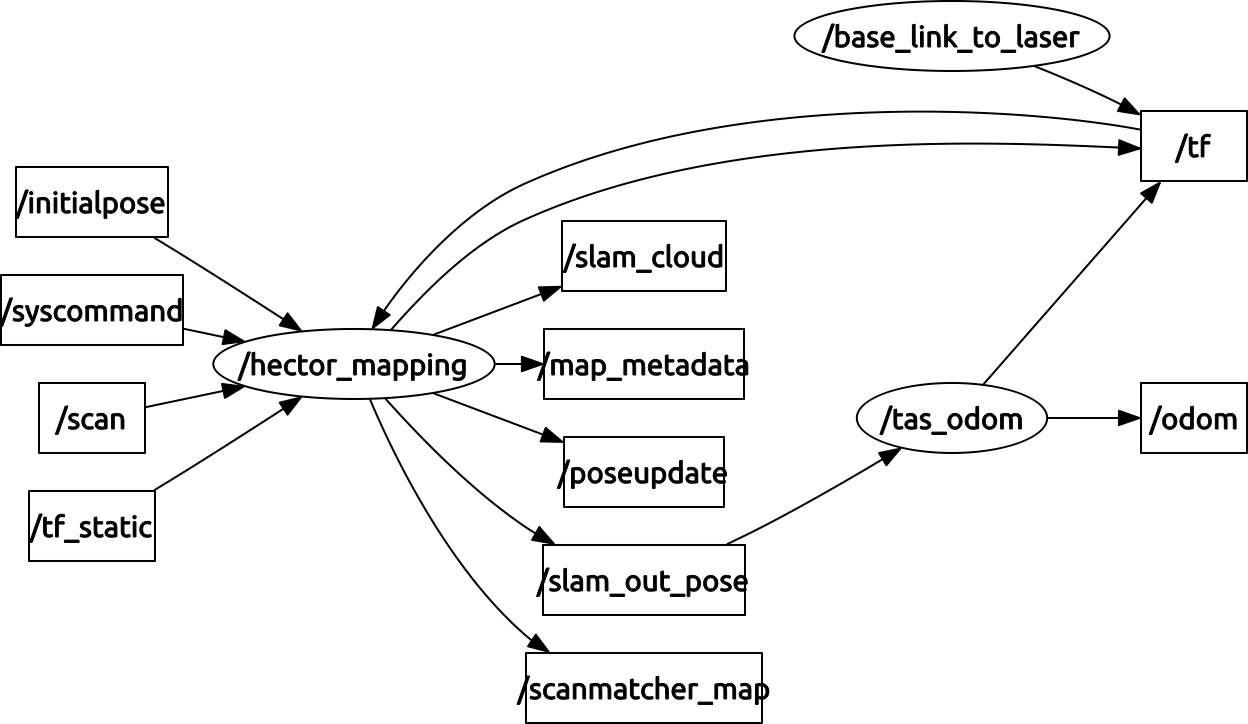
\includegraphics[width=0.9\textwidth]{diagrams/rqt_odom}
	\caption{Overview of the TAS-Odometry}
	\label{fig:rqt_odom}
\end{figure}

Currently there is no real odometry on the car available. For the navigation packages though odometry data is required (see picture \reffig{move_base_overview}). This was solved by using of a "fake-odometry". We take position and orientation estimated from the laserscanner data, and provide them as odometry data to the navigation package. 

To launch the fake odometry open a terminal and run the odom.launch file:

\shellcmd{roscd tas/launch} \\
\shellcmd{roslaunch odom.launch}

Picture \reffig{rqt_odom} shows the running nodes and topics for the fake odometry.

\subsection{hector\_mapping}
\label{sec:tas_package_odom_hector}

The hector\_mapping node implements a SLAM-algorithm \footnote{Simultaneous Localization and Mapping} to build a map and localize the car in it simultaneously at runtime. In picture \reffig{hector_buidling_process} you can see the building process. It shows the created map at three different timesteps.

\begin{figure}[h]
	\centering
		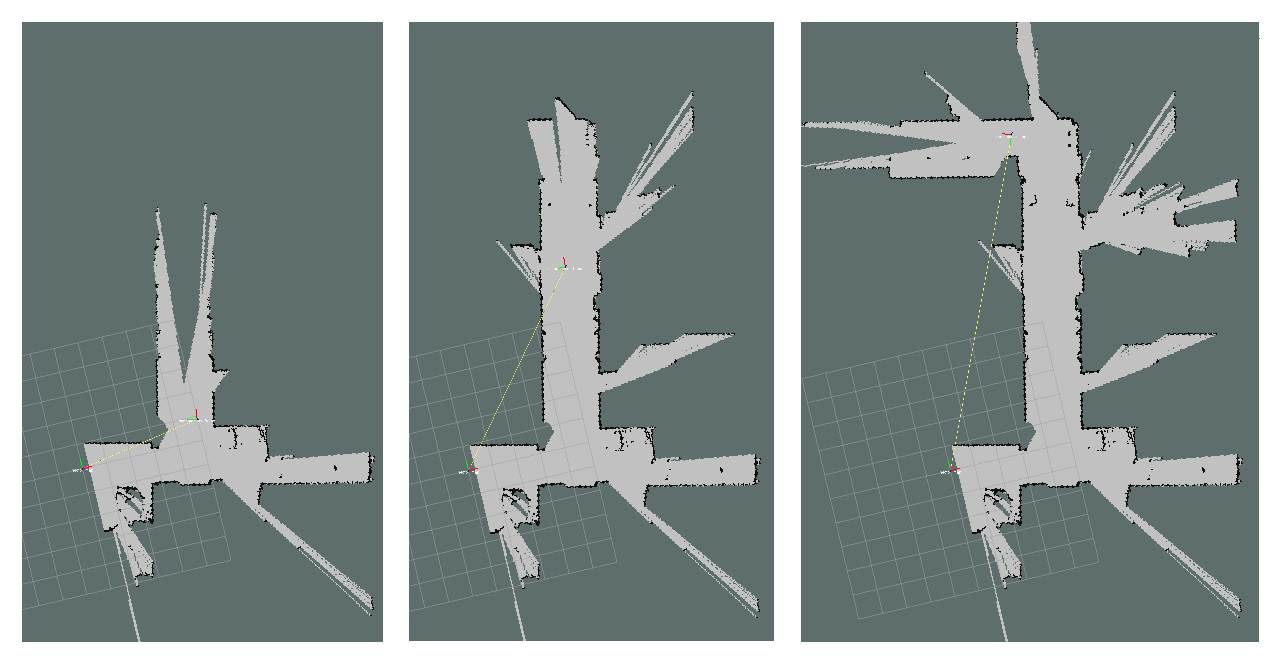
\includegraphics[width=\textwidth]{hector}
	\caption{Building process of a map with hector\_mapping}
	\label{fig:hector_buidling_process}
\end{figure}

Unlike other solutions for localization (see the \texttt{amcl package} in section \refsec{tas_package_amcl}) it only needs data from the laserscanner and does not require any odometry inputs. This is the reason why we use it to provide the fake odometry.

The estimated position and orientation is published to the \texttt{/poseupdate} (with covariance) and the \texttt{/slam\_out\_pose} topics (without covariance). 
 
For correct position estimation the node needs information about the relation between coordinate frame of the laserscanner and the coordinate frame of the car (refer to the next section \refsec{tas_package_transformations} for an introduction to transformations and frames). 

For more details about the parameters and settings of the package see:

\hyperref[http://wiki.ros.org/hector_mapping]{http://wiki.ros.org/hector\_mapping}

\section{Transformations}
\label{sec:tas_package_transformations}

\newpage
\section{Navigation}
\label{sec:tas_package_navigation}

\begin{figure}[h]
	\centering
		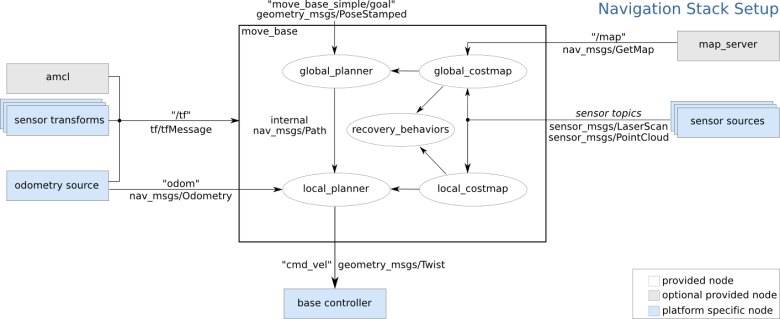
\includegraphics[width=\textwidth]{move_base_overview}
	\caption{Basic Navigation Stack}
	\label{fig:move_base_overview}
\end{figure}

In ROS in general the Navigation Stack takes sensor inputs from odometry, laser and other sources and outputs velocity commands to reach a given goal. Picture \reffig{move_base_overview} shows the parts of the basic Navigation Stack which is installed on the car.

To run the Navigation Stack open a terminal and type in:

\shellcmd{roscd tas/launch}\\
\shellcmd{roslaunch move\_base.launch}

The launch file will run all necessary parts of the Stack. Keep in mind that the hardware drivers and the TAS-Odometry package have to be launched before (see \refsec{tas_package_drivers} for hardware drivers and \refsec{tas_package_odom} for odometry).

To specify a goal for the car you can use the visualization tool RVIZ. Open a terminal and type in:

\shellcmd{roscd tas/launch} \\
\shellcmd{rosrun rviz rviz -d config/rviz/tas\_rviz.rviz}

This will run rviz with the configuration file in the \texttt{config} directory. At the beginning you have to give an initial estimation of the position to the \texttt{amcl node}. After that you can give goals to the \texttt{move\_base node} which the car will try to reach (see the marked buttons in picture \reffig{rviz_estimation}). To actually drive the car you have to push the \texttt{C-button} on the wii-nunchuk. 

\begin{figure}[h]
	\centering
		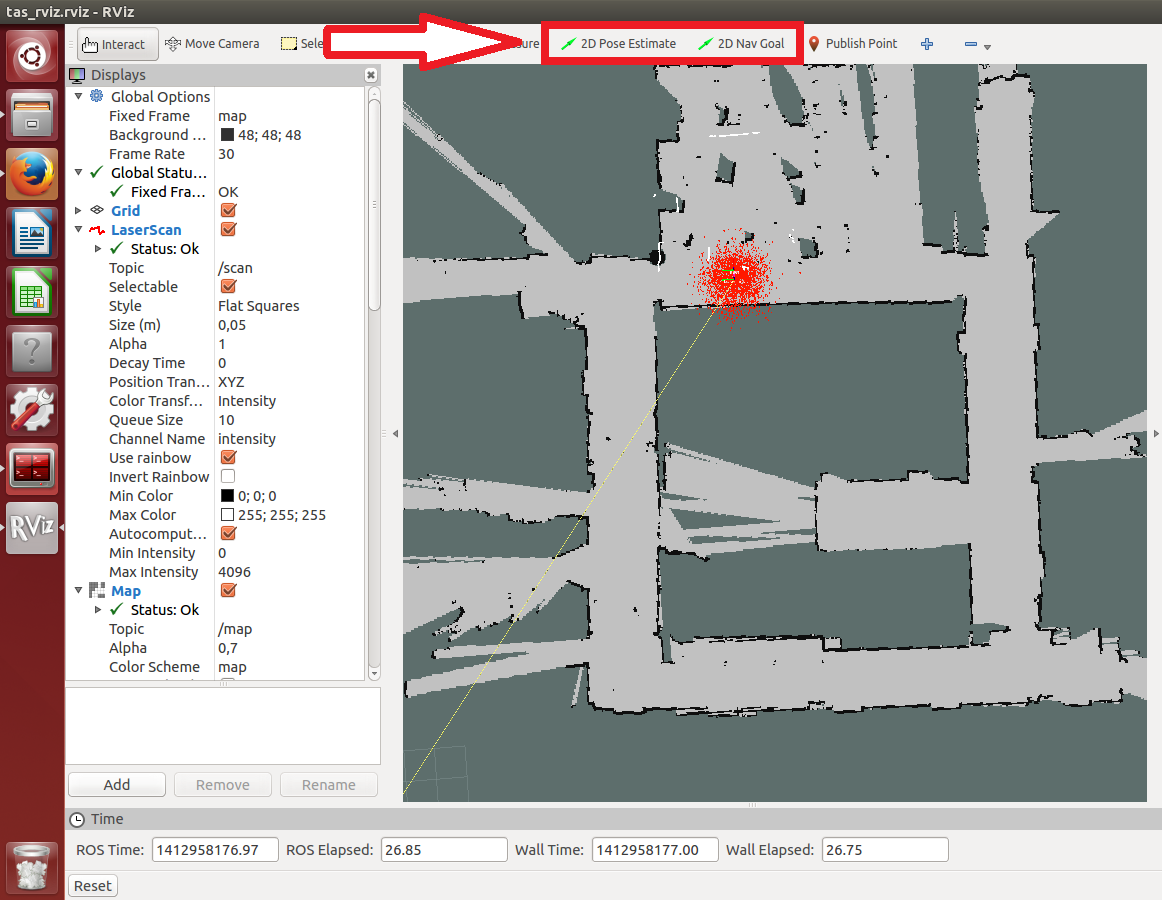
\includegraphics[width=\textwidth]{rviz_estimation}
	\caption{RVIZ visualization tool}
	\label{fig:rviz_estimation}
\end{figure}


Alternately you can launch hardware drivers, TAS-Odometry, the Navigation Stack and the RVIZ tool at once by launching the \texttt{run\_rviz.launch} file.

\subsection{map\_server}
\label{sec:tas_package_map_server}
The \texttt{map\_server} node takes a 2-D map of the environment and provides it as a ROS-service to other nodes. For every map there has to be a configuration file. The map file and the configuration file are located in the \texttt{config} directory of the TAS-package (see picture \reffig{tas_folder_struct} for the folder structure). The path of these files can be changed in the launchfile. For more information about the parameters of the \texttt{map\_server} package refer to:

\hyperref[http://wiki.ros.org/map_server]{http://wiki.ros.org/map\_server}


\subsection{amcl}
\label{sec:tas_package_amcl}
The \texttt{amcl} node implements different Monte Carlo localization algorithms to estimate the position of the robot. It requires a laserscanner, odometry and a map of the environment. The position and orientation with it's covariances is published to the \texttt{/amcl\_pose} topic.

The node takes odometry data in form of the transformation between the odometry frame and the coordinate frame of the car. See section \refsec{tas_package_transformations} for information about the \texttt{tf package}. Refer also to the package documentation on:

\hyperref[http://wiki.ros.org/amcl]{http://wiki.ros.org/amcl}



\subsection{move\_base}
\label{sec:tas_package_move_base}

The \texttt{mode\_base} implements a local and a global planner to calculate velocity commands to reach the navigation goal. These commands are published to the \texttt{/cmd\_vel} topic which is a general interface to the hardware of the robot. In our case the commands are taken by the \texttt{autonomous\_control} node to get the car moving (see next section \refsec{tas_package_autonomous_control}).

In the \texttt{config} folder (see picture \reffig{tas_folder_struct}) there are several configuration files for the planners. For information about settings and parameters refer to:

\hyperref[http://wiki.ros.org/move_base?distro=indigo]{http://wiki.ros.org/move\_base?distro=indigo}

\subsection{tas\_autonomous\_control}
\label{sec:tas_package_autonomous_control}
The  \texttt{autonomous\_control} node mainly takes the velocity commands generated by the \texttt{move\_base} node and publishes the corresponding PWM values for the motor controllers to the \texttt{/servo} topic.

For safety reasons the car only drives autonomously if the \texttt{C-button} on the wii-nunchuk is pressed.

Pay attention, that currently there are only two discrete velocity states implemented. See the following extract from the source code of the node:

\begin{lstlisting}
if(autonomous_control.cmd_linearVelocity>0) {
	autonomous_control.control_servo.x = 1550;
}

else if(autonomous_control.cmd_linearVelocity<0) {
	autonomous_control.control_servo.x = 1300;
}

else {
	autonomous_control.control_servo.x = 1500;
}

autonomous_control.control_servo.y = 
 autonomous_control.cmd_steeringAngle;
\end{lstlisting}












%
% Beispielkapitel: Bedienung dieser Vorlage
%

% Zum Setzen von TeX-Quellcode, der nicht interpretiert werden soll
\newcommand{\makro}[1]{\texttt{\textbackslash{}#1\{\}}}

\chapter{Additional topics}
\label{sec:advanced}


\section{Shell scripts}
\label{sec:advanced_shell_scripts}

\section{External RVIZ}
\label{sec:advanced_rviz_ext}

\section{VNC}
\label{sec:advanced_vnc}

\section{Recording and playing data}
\label{sec:advanced_rosbag}

\section{Integrated Development Environments (IDE's)}
\label{sec:advanced_ide}

\section{Version control with git}
\label{sec:advanced_git}

\section{Arduino code}
\label{sec:advanced_ide}
\todo{Put arduino code in repository}

\section{Switching remote controller}
\label{sec:advanced_switch}

% === Anhang ===
\appendix
% Anhang
%%
% Kapitel: Anhang
%

\clearpage
\addcontentsline{toc}{chapter}{Anhang}


\chapter{Was geh�rt in den Anhang?}
Z.\,B. l�ngere mathematische Herleitungen, Datenbl�tter von verwendeten Komponenten, ausf�hrliche Auflistungen von (Zwischen-)Ergebnissen und alles, was nicht direkt den roten Faden der Arbeit bildet


% Literaturverzeichnis
\nocite{*} % hiermit werden auch nichtzitierte Quellen ins Literaturverzeichnis aufgenommen
\bibliography{literature} % am besten die aus dem SVN

% TODO-Liste: alle im Text mit \todo{} angemerkten Stellen werden hier aufgef�hrt
% Sollten keine mehr vorhanden sein, wird die Liste ausgeblendet
\ifthenelse{\thetodo > 0}{
	\pdfbookmark[0]{\todolistname}{tod}
	\listoftodo
}{}

\end{document}

%
% EOF
%